\def\linkdethi{} %Đường link cần dẫn tới
\anmaQR
%%%%%%%%%%%%%%%%%%%%%%%%
\def\toanlop{12}
\def\thoigian{90}
\def\namhoc{2025 - 2026}
\begin{dethi}
	{Bộ GD\&ĐT}
	{VTED ft KING EDU}
	{TDMZD03}
	{Đề thi thử THPTQG 2026}
\end{dethi}
\caulc
\Opensolutionfile{ans}[ans/ansTN-Dung]
%%%=============EX_1=============%%%
\begin{ex}%[1D2N3-4]%[TDMZD03]%[Mui Doan]
	Cho cấp số nhân $(u_n)$ có $u_1=2$ và $u_2=1$. Giá trị của $u_3$ bằng
	\choice
	{$4$}
	{$2$}
	{$8$}
	{\True $\dfrac{1}{2}$}
	\loigiai{
		Ta có công bội của cấp số nhân là $q=\dfrac{u_2}{u_1}=\dfrac{1}{2}$.\\
		Giá trị của $u_3$ là $u_3=u_1 \cdot q^2=2\cdot \left(\dfrac{1}{2}\right)^2=2\cdot\dfrac{1}{4}=\dfrac{1}{2}$.
	}
\end{ex}
%%%=============================%%%

%%%=============EX_2=============%%%
\begin{ex}%[1H8H7-1]%[TDMZD03]%[Huỳnh Trí Thiện]
	Cho khối chóp có diện tích đáy bằng $3$ và chiều cao bằng $2$. Thể tích của khối chóp này bằng
	\choice
	{$6$}
	{$5$}
	{$18$}
	{\True $2$}
	\loigiai{
		Thể tích của khối chóp là \[V = \dfrac{1}{3} S \cdot h  = \dfrac{1}{3} \cdot 3 \cdot 2 = 2.\]
		Vậy thể tích của khối chóp bằng $2$.
	}
\end{ex}
%%%=============================%%%

%%%=============EX_3=============%%%
\begin{ex}%[1D6N3-2]%[TDMZD03]%[Chu Hà]
	Tập xác định của hàm số $y=\left(3x-x^2\right)^{0,5}$ là
	\choice
	{$(0;+\infty)$}
	{\True $(0;3)$}
	{$\mathbb{R}\setminus\{0;3\}$}
	{$[0;3]$}
	\loigiai{
		Hàm số $y=\left(3x-x^2\right)^{0,5}$ có số mũ $\alpha = 0{,}5$ là số không nguyên.\\
		Do đó, điều kiện xác định của hàm số là cơ số phải dương
		\[3x-x^2>0 \Leftrightarrow 0 < x < 3 \Leftrightarrow x\in (0;3).\]
		Vậy tập xác định của hàm số là $\mathscr{D}=(0;3)$.
	}
\end{ex}
%%%=============================%%%

%%%=============EX_4=============%%%
\begin{ex}%[1D6N4-5]%[TDMZD03]%[Nguyễn Tấn Linh]
	Tập nghiệm của bất phương trình $\log_3(x-1)<2$ là
	\choice
	{\True $(1;10)$}
	{$(0;1)$}
	{$(9;+\infty)$}
	{$(10;+\infty)$}
	\loigiai{
		Điều kiện xác định $x-1>0 \Leftrightarrow x>1$.\\
		Vì cơ số $3>1$ nên bất phương trình đã cho tương đương với
		\[x-1<3^2 \Leftrightarrow x-1<9 \Leftrightarrow x<10.\]
		Kết hợp với điều kiện $x>1$, ta được $1<x<10$.\\
		Vậy tập nghiệm của bất phương trình là $(1;10)$.
	}
\end{ex}
%%%=============================%%%

%%%=============EX_5=============%%%
\begin{ex}%[2D1N1-2]%[TDMZD03]%[Phạm Hải Dương]
	Cho bảng biến thiên của hàm số $f(x)$ như hình vẽ bên dưới. Hỏi hàm số $f(x)$ nghịch biến trên khoảng nào, trong các khoảng dưới đây?
	\begin{center}
		\begin{tikzpicture}[font=\normalsize,t style/.style={style=solid}]
			\tkzTabInit[nocadre=false,lgt=1.2,espcl=2.5,deltacl=0.5]
			{$x$/0.75,$f'(x)$/0.75,$f (x)$/3}
			{$-\infty$,$-3$,$0$,$3$,$+\infty$}
			\tkzTabLine{,-,0,+,0,-,0,+}
			\path
			($(N13)!0.8!(N12)$) node (A1){$ +\infty $}
			($(N23)!0.1!(N22)$) node (A2){$ -2 $}
			($(N33)!0.6!(N32)$) node (A3){$ 1 $}
			($(N43)!0.1!(N42)$) node (A4){$ -2 $}
			($(N53)!0.8!(N52)$) node (A5){$ +\infty $};
			\foreach \x/\y in {A1/A2,A2/A3,A3/A4,A4/A5}{
				\draw[-stealth] (\x)--(\y);
			}
		\end{tikzpicture}
	\end{center}
	\choice
	{$(-\infty;-2)$}
	{$(-3;0)$}
	{\True $(0;3)$}
	{$(3;+\infty)$}
	\loigiai{
		Dựa vào bảng biến thiên, ta thấy $f'(x) < 0$ trên các khoảng $(-\infty; -3)$ và $(0; 3)$.\\
		Do đó, hàm số $f(x)$ nghịch biến trên các khoảng $(-\infty; -3)$ và $(0; 3)$.
	}
\end{ex}
%%%=============================%%%

%%%=============EX_6=============%%%
\begin{ex}%[2D4H1-2]%[TDMZD03]%[Nguyễn Sơn Thành]
	Cho hàm số $f(x)=2x-3$. Trong các khẳng định sau, khẳng định nào \textbf{đúng}?
	\choice
	{$\displaystyle\int f(x) \mathrm{d}x = 2x^2-3x+C$}
	{$\displaystyle\int f(x) \mathrm{d}x = x^2-3+C$}
	{$\displaystyle\int f(x) \mathrm{d}x = -x+C$}
	{\True $\displaystyle\int f(x) \mathrm{d}x = x^2-3x+C$}
	\loigiai{
		Ta có $\displaystyle\int f(x) \mathrm{d}x = \int (2x-3) \mathrm{d}x = x^2-3x+C$.
	}
\end{ex}
%%%=============================%%%

%%%=============EX_7=============%%%
\begin{ex}%[2H5N3-2]%[TDMZD03]%[Bồ Văn Hậu]
	Trong không gian $Oxyz$, mặt cầu $(S)\colon x^2+y^2+z^2-2z-4y=0$ có tọa độ tâm là
	\choice
	{$(0;1;2)$}
	{$(0;2;4)$}
	{$(0;4;2)$}
	{\True $(0;2;1)$}
	\loigiai{
		Phương trình mặt cầu $(S)$ có dạng $x^2+y^2+z^2-2ax-2by-2cz+d=0$.\\
		Từ phương trình $(S)\colon x^2+y^2+z^2-4y-2z=0$, ta có
		\[\heva{&-2a = 0 \\&-2b = -4 \\&-2c = -2} \Leftrightarrow \heva{&a = 0 \\&b = 2 \\&c = 1.}\]
		Vậy mặt cầu $(S)$ có tâm là $I(0;2;1)$.
	}
\end{ex}
%%%=============================%%%

%%%=============EX_8=============%%%
\begin{ex}%[2H2H1-2]%[TDMZD03]%[Lê Phúc]
	\immini[thm]{Cho hình chóp đều $S.ABCD$. Đáp án \textbf{đúng} là
		\choice
		{\True $\overrightarrow{SA}-\overrightarrow{SB}=\overrightarrow{SD}-\overrightarrow{SC}$}
		{$\overrightarrow{SA}+\overrightarrow{SB}=\overrightarrow{SC}+\overrightarrow{SD}$}
		{$\overrightarrow{SA}+\overrightarrow{SB}+\overrightarrow{SC}+\overrightarrow{SD}=\overrightarrow{0}$}
		{$\overrightarrow{DA}+\overrightarrow{BS}+\overrightarrow{SC}=\overrightarrow{SA}$}}
	{
		\begin{tikzpicture}[font=\scriptsize]
			\tikzset{declare function={a=3; b=2; h=2.5;}}
			\path (0,0) coordinate (A)
			(a,0) coordinate (D)
			(-135:b) coordinate (B)
			($(B)+(D)$) coordinate (C)
			($(A)!0.5!(C)$) coordinate (O)
			($(O)+(0,h)$) coordinate (S);
			\path pic[draw,angle radius=3pt]{right angle=A--O--S};
			\path pic[draw,angle radius=3pt]{right angle=D--O--S};
			\draw[dashed] (B)--(A)--(D)--cycle (C)--(A)--(S)--(O);
			\draw (S)--(B)--(C)--(D)--cycle (S)--(C);
			\foreach \t/\g in {A/150,B/-90,C/-60,D/60,S/90,O/-90}{
				\fill (\t) circle (1pt) node[shift={(\g:7pt)},font=\scriptsize]{$\t$};
			}
		\end{tikzpicture}
	}
	\loigiai{
		Gọi $O$ là tâm của mặt đáy $ABCD$, suy ra $O$ là trung điểm của $AC$ và $BD$.\\ Xét từng mệnh đề
		\begin{itemize}
			\item  $\overrightarrow{SA}-\overrightarrow{SB}=\overrightarrow{SD}-\overrightarrow{SC}$\\
			Theo quy tắc hiệu vectơ, ta có $\overrightarrow{SA}-\overrightarrow{SB}=\overrightarrow{BA}$ và $\overrightarrow{SD}-\overrightarrow{SC}=\overrightarrow{CD}$.\\
			Vì $ABCD$ là hình vuông nên $\overrightarrow{BA}=\overrightarrow{CD}$.
			\item  $\overrightarrow{SA}+\overrightarrow{SB}=\overrightarrow{SC}+\overrightarrow{SD}$\\
			Ta có $\overrightarrow{SA}+\overrightarrow{SB}=\overrightarrow{SC}+\overrightarrow{SD} \Leftrightarrow \overrightarrow{SA}-\overrightarrow{SC}=\overrightarrow{SD}-\overrightarrow{SB} \Leftrightarrow \overrightarrow{CA}=\overrightarrow{BD}$.\\
			Vì hai vectơ $\overrightarrow{CA}$ và $\overrightarrow{BD}$ không cùng phương nên mệnh đề này \textbf{sai}.
			\item  $\overrightarrow{SA}+\overrightarrow{SB}+\overrightarrow{SC}+\overrightarrow{SD}=\overrightarrow{0}$\\
			Ta có $\left(\overrightarrow{SA}+\overrightarrow{SC}\right)+\left(\overrightarrow{SB}+\overrightarrow{SD}\right) = 2\overrightarrow{SO}+2\overrightarrow{SO}=4\overrightarrow{SO} \ne \overrightarrow{0}$.
			\item  $\overrightarrow{DA}+\overrightarrow{BS}+\overrightarrow{SC}=\overrightarrow{SA}$\\
			Theo quy tắc ba điểm, ta có $\overrightarrow{BS}+\overrightarrow{SC}=\overrightarrow{BC}$.\\
			Mặt khác, vì $ABCD$ là hình vuông nên $\overrightarrow{BC}=\overrightarrow{AD}$.\\
			Suy ra $\overrightarrow{DA}+\overrightarrow{BS}+\overrightarrow{SC} = \overrightarrow{DA}+\overrightarrow{AD}=\overrightarrow{0} \ne \overrightarrow{SA}$.
		\end{itemize}
	}
\end{ex}
%%%=============================%%%

%%%=============EX_9=============%%%
\begin{ex}%[1D5H1-2]%[TDMZD03]%[Trần Văn Thiện]
	Cho mẫu số liệu ghép nhóm $M$ có tất cả $10$ nhóm với độ dài bằng nhau.
	Biết rằng đầu mút phải của nhóm thứ $n$ có giá trị bằng đầu mút trái của nhóm thứ ($n+1$), đầu mút trái của nhóm thứ $7$ nhiều hơn đầu mút phải của nhóm thứ $2$ là $6$ đơn vị. Hãy xác định khoảng biến thiên của mẫu số liệu $M$.
	\choice
	{$12$}
	{\True $15$}
	{$24$}
	{$10,8$}
	\loigiai{
		Giả sử các nhóm của mẫu số liệu là $[a_1; a_2)$, $[a_2; a_3)$, $\ldots$, $[a_{10}; a_{11})$.\\
		Gọi $d$ là độ dài của mỗi nhóm, ta có $d = a_{i+1} - a_i$ với mọi $i = 1$, $2$, $\ldots$, $10$.\\
		Đầu mút trái của nhóm thứ $7$ là $a_7$, đầu mút phải của nhóm thứ $2$ là $a_3$.\\
		Theo giả thiết, $a_7 - a_3 = 6 \Leftrightarrow 4d = 6 \Leftrightarrow d = 1{,}5$.\\
		Độ dài của mỗi nhóm là $1{,}5$ đơn vị.\\
		Vậy khoảng biến thiên của mẫu số liệu ghép nhóm $M$ là $R = a_{11} - a_1 = 10d = 10 \cdot 1{,}5 = 15$.
	}
\end{ex}
%%%=============================%%%

%%%=============EX_10=============%%%
\begin{ex}%[2H5H1-3]%[TDMZD03]%[Đình Nguyên]
	Trong không gian $Oxyz$, cho ba điểm có tọa độ $A(1;2;0)$, $B(-2;1;1)$, $C(3;0;-2)$. Phương trình mặt phẳng đi qua $A$, vuông góc với đường thẳng $BC$ là
	\choice
	{\True $5x-y-3z-3=0$}
	{$x+y-z-3=0$}
	{$2x-y-z=0$}
	{$4x-3y-3z+2=0$}
	\loigiai{
		Đường thẳng $BC$ có vectơ chỉ phương là $\overrightarrow{BC}=(5;-1;-3)$.\\
		Phương trình mặt phẳng cần tìm đi qua điểm $A(1;2;0)$ và nhận $\overrightarrow{BC}=(5;-1;-3)$ làm vectơ pháp tuyến là
		\[5(x-1)-1(y-2)-3(z-0)=0 \Leftrightarrow 5x-y-3z-3=0.\]
	}
\end{ex}
%%%=============================%%%

%%%=============EX_11=============%%%
\begin{ex}%[2D4H3-3]%[TDMZD03]%[Huynh Quốc Đạt]
	Cho hình phẳng $(H)$ giới hạn bởi $f(x)=x^2-6x$, trục hoành $Ox$. Khi cho hình phẳng $(H)$ quay quanh trục $Ox$ thì thể tích khối tròn xoay thu được là
	\choice
	{$36\pi$}
	{$\dfrac{2\,218\pi}{3}$}
	{$84\pi$}
	{\True $\dfrac{1\,296\pi}{5}$}
	\loigiai{
		Phương trình hoành độ giao điểm của đồ thị hàm số $f(x)$ và trục hoành
		\[x^2-6x=0\Leftrightarrow \hoac{&x=0\\ &x=6.}\]
		Thể tích khối tròn xoay thu được khi quay hình phẳng $(H)$ quanh trục $Ox$ là
		\[V=\pi \displaystyle\int\limits_{0}^{6}\left(x^2-6x\right)^2\mathrm{d}x=\dfrac{1\,296\pi}{5}.\]
	}
\end{ex}
%%%=============================%%%

%%%=============EX_12=============%%%
\begin{ex}%[2D1H3-2]%[TDMZD03]%[Nguyễn Trí Minh Tuấn] 
	Giá trị lớn nhất và nhỏ nhất của hàm số $y=\dfrac{x^2+2x+1}{x^2-4x+5}$ lần lượt là
	\choice
	{$5$ và $-1$}
	{\True $10$ và $0$}
	{$\dfrac{7}{3}$ và $-1$}
	{$6$ và $0$}
	\loigiai{
		Tập xác định của hàm số là $\mathscr{D} = \mathbb{R}$ (vì $x^2-4x+5 = (x-2)^2+1 > 0$ với mọi $x \in \mathbb{R}$).\\
		Ta có 
		\[y'=\dfrac{(2x+2)(x^2-4x+5)-(x^2+2x+1)(2x-4)}{(x^2-4x+5)^2} = \dfrac{-6x^2+8x+14}{(x^2-4x+5)^2}.\]
		Khi đó $y'=0 \Leftrightarrow -6x^2+8x+14=0 \Leftrightarrow \hoac{&x=-1\\& x=\dfrac{7}{3}.}$\\
		Bảng biến thiên
		\begin{center}
			\begin{tikzpicture}[font=\normalsize,t style/.style={style=solid}]
				\tkzTabInit[nocadre=false,lgt=1.5,espcl=2.6,deltacl=0.65]
				{$x$/1.2, $f'(x)$/0.75, $f (x)$/3} 
				{$-\infty$,$-1$,$\dfrac{7}{3}$,$+\infty$} 
				\tkzTabLine{,-,0,+,0,-}
				\path
				($(N13)!0.5!(N12)$) node (A1){$ 1 $}
				($(N23)!0.1!(N22)$) node (A2){$ 0 $}
				($(N33)!0.8!(N32)$) node (A3){$ 10 $}
				($(N43)!0.5!(N42)$) node (A4){$ 1 $};
				\foreach \x/\y in {A1/A2,A2/A3,A3/A4}{
					\draw[-stealth] (\x)--(\y);
				}
			\end{tikzpicture}
		\end{center}
		Dựa vào bảng biến thiên, ta có $\min\limits_{\mathbb{R}} y=0$ tại $x=-1$ và $\max\limits_{\mathbb{R}} y=10$ tại $x=\dfrac{7}{3}$.
	}
\end{ex}
%%%=============================%%%
\Closesolutionfile{ans}

\cauds
\Opensolutionfile{ans}[ans/ansTN-DungSai]
%%%=============EX_13=============%%%
\begin{ex}%[2D1V2-1]%[TDMZD03]%[Dương Công Tạo]
	Cho hàm số $f(x) = 2x^2 - \cos2x$. Gọi $F(x)$ là một nguyên hàm của hàm số $f(x)$. Biết rằng đồ thị hàm số $y = f'(x)$ và đồ thị hàm số $y = F(x)$ có cùng tâm đối xứng.
	\choiceTF[t]
	{\True $f'(x) = 4x + 2\sin2x$}
	{\True Tâm đối xứng của đồ thị hàm số $y = f'(x)$ là gốc toạ độ $O$}
	{$F(x) = \dfrac{2}{3}x^3-2\sin2x$}
	{\True Đồ thị của hàm số $y = F(x)$ có hai điểm cực trị nằm về hai phía của $Oy$}
	\loigiai{
		\begin{itemchoice}
			\itemch Ta có $f(x) = 2x^2 - \cos2x$.\\ Suy ra $f'(x) = 4x+2\sin2x$.
			\itemch Xét hàm số $f'(x) = 4x+2\sin2x$ có tập xác định $\mathscr{D}=\mathbb{R}$.\\
			Ta có $\forall x\in \mathscr{D}\Rightarrow -x\in \mathscr{D}$ và $f'(-x)=4(-x)+2\sin(-2x)=-(4x+2\sin 2x)=-f'(x)$.\\
			Suy ra $f'(x)$ là hàm số lẻ. Do đó, đồ thị hàm số $y = f'(x)$ nhận gốc toạ độ $O$ là tâm đối xứng.
			\itemch Vì $F(x)$ là một nguyên hàm của hàm số $f(x)$ nên 
			\[F(x)=\displaystyle\int f(x)\,\mathrm{d}x=\displaystyle\int \left(2x^2 - \cos2x\right)\,\mathrm{d}x=\dfrac{2}{3}x^3-\dfrac{1}{2}\sin 2x+C.\]
			Vì đồ thị hàm số $y = f'(x)$ và đồ thị hàm số $y = F(x)$ có cùng tâm đối xứng là gốc tọa độ $O$ nên đồ thị hàm số $y = F(x)$ đi qua $O(0;0)$, suy ra
			\[F(0)=0\Leftrightarrow C=0.\]
			Vậy $F(x)=\dfrac{2}{3}x^3-\dfrac{1}{2}\sin 2x$.
			\itemch 
			Ta có $F'(x) = f(x) = 2x^2 - \cos 2x$.\\ Để giải phương trình $F'(x)=f(x)=0$, ta phải xét các đạo hàm cấp một và cấp hai của $f(x)$ như sau
			$f'(x) = 4x + 2\sin 2x$; $f''(x) = (4x + 2\sin 2x)' = 4 + 4\cos 2x \ge 0$.\\
			Ta có bảng biến thiên của hàm số
				\begin{center}
					\begin{tikzpicture}[>=stealth,line join=round,line cap=round,every node/.style={font=\scriptsize},declare function={d=15pt;}]
						\tkzTabInit[nocadre=false,lgt=1.5,espcl=2.5,deltacl=0.6]
						{$x$/1.0,$f''(x)$/1.0,$f'(x)$/2.5,$f (x)$/3.5}
						{$-\infty$,$x_1$,$0$,$x_2$,$+\infty$}
						\foreach \i in {2,3,4}{
							\draw[white,line width=1.5pt] (N\i1) -- (N\i4);
							\draw[dashed,line width=0.6pt] (N\i1) -- (N\i4);
						}
						\node at ($(N11)!0.5!(N22)$) {$\ge 0$};
						\node at ($(N41)!0.5!(N52)$) {$\ge 0$};
						\coordinate (C) at ($(N32)!0.5!(N33)$);
						\draw[dashed,red] (N12|-C) -- (N52|-C) node[above left,inner sep=2pt] {$y=0$};
						\coordinate (P1) at ([yshift=d]N13);
						\coordinate (P2) at ([yshift=-d]N52);
						\draw[-stealth] (P1) -- (P2);
						\fill (C) circle (1.5pt);
						\coordinate (Mid1) at ($(N12)!0.5!(N22)$);
						\coordinate (Mid4) at ($(N42)!0.5!(N52)$);
						\coordinate (V1) at (Mid1|-N14);
						\coordinate (Slant1) at (intersection of P1--P2 and Mid1--V1);
						\coordinate (Dash1) at (Mid1|-C);
						\node at ($(Slant1)!0.5!(Dash1)$) {$-$};
						\coordinate (V4) at (Mid4|-N14);
						\coordinate (Slant4) at (intersection of P1--P2 and Mid4--V4);
						\coordinate (Dash4) at (Mid4|-C);
						\node at ($(Slant4)!0.5!(Dash4)$) {$+$};
						\path
						([yshift=-d]N13) node (A1) {$+\infty$}
						([yshift=d]N34) node (A3) {$-1$}
						([yshift=-d]N53) node (A5) {$+\infty$};
						\draw[-stealth] (A1) -- (A3);
						\draw[-stealth] (A3) -- (A5);
						\coordinate (M1) at (intersection of A1.center--A3.center and N23--N24);
						\coordinate (M2) at (intersection of A3.center--A5.center and N43--N44);
						\draw[dashed,red] (N13|-M1) -- (N53|-M1) node[above left,inner sep=2pt] {$y=0$};
						\fill (M1) circle (1.5pt);
						\fill (M2) circle (1.5pt);
					\end{tikzpicture}
				\end{center}
			Đạo hàm của hàm số $F(x)$ là $f(x)$ đổi dấu khi qua các nghiệm $x_1 < 0 < x_2$, suy ra đồ thị hàm số $y=F(x)$ có hai điểm cực trị nằm ở hai phía trục tung $Oy$.
		\end{itemchoice}
	}
\end{ex}
%%%=============================%%%

%%%=============EX_14=============%%%
\begin{ex} %[2D4V2-6]%[TDMZD03]%[Hà Văn Hảo]
	Một đoàn tàu dài $150$\,m đang chuyển động thẳng đều trên một đường ray với tốc độ $30$\,m/s thì thấy ở phía trước $600$\,m so với đầu tàu $A$ có đầu $C$ của một chiếc cầu dài $270$\,m. Người lái tàu ngay sau đó $5$ giây bắt đầu cho tàu giảm tốc độ theo gia tốc $a(t) = -bt$\,(m/s$^2$), với $t$ tính theo giây và là thời gian tính từ lúc bắt đầu giảm tốc, $b$ là số thực dương. Biết rằng sau khi giảm tốc được $12$ giây thì đầu tàu đến điểm $D$ và đạt tốc độ $8$\,m/s. Tại $D$ bắt đầu cho tàu chuyển động đều để đi qua cầu cho an toàn.
	\choiceTF[t]
	{\True Tại thời điểm bắt đầu giảm tốc đầu tàu cách $C$ một đoạn bằng $450$\,m}
	{$b = 0{,}5$}
	{\True $DC=178$\,m}
	{Tổng thời gian tính từ lúc bắt đầu giảm tốc tới khi tàu đi qua được cầu là $68$ giây}
	\loigiai{
		\begin{center}
			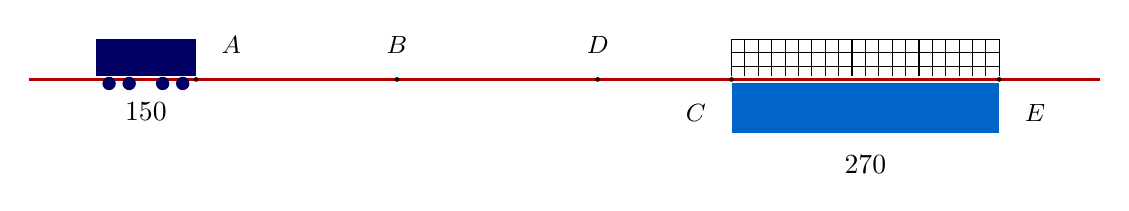
\begin{tikzpicture}[font=\small, >=stealth, scale=0.85]
				\definecolor{darkblue}{RGB}{0, 0, 100}
				\definecolor{bridgeblue}{RGB}{0, 100, 200}
				\definecolor{trackred}{RGB}{180, 0, 0}
				\draw[thick, trackred] (0,0) -- (16,0);			
				\fill (2.5, 0) circle (1pt) node[above right=0.2cm] {$A$};
				\fill (5.5, 0) circle (1pt) node[above=0.2cm] {$B$};
				\fill (8.5, 0) circle (1pt) node[above=0.2cm] {$D$};
				\fill (10.5, 0) circle (1pt) node[below left=0.2cm] {$C$};
				\fill (14.5, 0) circle (1pt) node[below right=0.2cm] {$E$};
				\begin{scope}[shift={(2.5,0)}]
					\fill[darkblue] (-1.3, -0.06) circle (0.1);
					\fill[darkblue] (-1.0, -0.06) circle (0.1);
					\fill[darkblue] (-0.5, -0.06) circle (0.1);
					\fill[darkblue] (-0.2, -0.06) circle (0.1);
					\fill[darkblue] (-1.5, 0.05) rectangle (0, 0.6);
					\node[below, font=\normalsize] at (-0.75, -0.2) {$150$};
				\end{scope}
				\begin{scope}[shift={(10.5,0)}]
					\draw[step=0.2cm, black, thin] (0, 0.05) grid (4, 0.6);
					\fill[bridgeblue] (0, -0.05) rectangle (4, -0.8);
					\node[below, font=\normalsize] at (2, -1.0) {$270$};
				\end{scope}
			\end{tikzpicture}
		\end{center}
		Gọi các điểm trên quỹ đạo của đầu tàu như hình vẽ
		\begin{itemize}
			\item $A$: Vị trí đầu tàu ban đầu.
			\item $B$: Vị trí đầu tàu lúc bắt đầu giảm tốc.
			\item $D$: Vị trí đầu tàu sau khi giảm tốc $12$ giây.
			\item $C$, $E$: Lần lượt là hai điểm đầu và cuối của chiếc cầu.
		\end{itemize}
		\begin{itemchoice}
			\itemch 
			Trong $5$ giây đầu, tàu chuyển động thẳng đều với vận tốc $v_0 = 30$\,m/s.\\
			Quãng đường đầu tàu đi được từ $A$ đến $B$ là $AB = 30 \cdot 5 = 150$\,(m).\\
			Khoảng cách ban đầu từ $A$ đến đầu cầu $C$ là $AC = 600$\,m.\\
			Tại thời điểm bắt đầu giảm tốc (đầu tàu tại $B$), khoảng cách đến cầu là
			\[BC = AC - AB = 600 - 150 = 450 \text{ (m)}.\]
			\itemch 
			Gia tốc của tàu là $a(t) = -bt$.\\ Vận tốc của tàu tại thời điểm $t$ kể từ lúc bắt đầu giảm tốc là
			\[v(t) = v_0 + \displaystyle\int\limits_0^t a(u)\mathrm{\,d}u = 30 + \displaystyle\int\limits_0^t (-bu)\mathrm{\,d}u = 30 - \dfrac{bt^2}{2}.\]
			Tại $D$ (tương ứng $t = 12$\,s), vận tốc đạt $v(12) = 8$\,m/s, ta có phương trình
			\[30 - \dfrac{b \cdot 12^2}{2} = 8 \Leftrightarrow 30 - 72b = 8 \Leftrightarrow 72b = 22 \Leftrightarrow b = \dfrac{11}{36} \approx 0{,}3055.\]
			\itemch 
			Quãng đường tàu di chuyển được trong $12$ giây giảm tốc (từ $B$ đến $D$) là
			\[BD = \displaystyle\int\limits_0^{12} v(t) \mathrm{\,d}t = \displaystyle\int\limits_0^{12} \left( 30 - \dfrac{11}{72}t^2 \right) \mathrm{\,d}t = \left( 30t - \dfrac{11}{216}t^3 \right) \Bigg|_0^{12} = 360 - 88 = 272 \text{ (m)}.\]
			Khoảng cách từ $D$ đến $C$ là
			\[DC = BC - BD = 450 - 272 = 178 \text{ (m)}.\]
			\itemch 
			Để tàu đi qua cầu an toàn, \textbf{đuôi của đoàn tàu} phải rời khỏi hoàn toàn điểm $E$ (đầu bên kia của cầu).\\
			Vì vậy, tổng quãng đường \textbf{đầu tàu} phải di chuyển tính từ điểm $D$ là
			\[s_3 = DC + CE + L_{\text{tàu}} = 178 + 270 + 150 = 598 \text{ (m)}.\]
			Thời gian để tàu đi hết quãng đường $s_3$ với vận tốc đều $v = 8$\,m/s là
			\[t_3 = \dfrac{s_3}{v} = \dfrac{598}{8} = 74{,}75 \text{ (s)}.\]
			Tổng thời gian tính từ lúc bắt đầu giảm tốc tới khi qua hết cầu là
			\[T = t_{\text{giảm tốc}} + t_3 = 12 + 74{,}75 = 86{,}75 \text{ (s)}.\]
		\end{itemchoice}
	}
\end{ex}
%%%=============================%%%

%%%=============EX_15=============%%%
\begin{ex}%[2D6V2-4]%[TDMZD03]%[Vũ Hồng Toàn]
	Hộp $A$ chứa bốn quả bóng được đánh số lần lượt là $1$, $2$, $3$, $4$. Hộp $B$ chứa ba quả bóng được đánh số $1$, $2$, $3$. Chọn ngẫu nhiên một trong hai hộp và sau đó chọn ngẫu nhiên một quả bóng từ hộp đó. Gọi $X$ là biến cố \lq\lq Hộp $A$ được chọn\rq\rq\, và $Y$ là biến cố \lq\lq Bóng số $2$ được chọn\rq\rq.
	\begin{center}
		\begin{tikzpicture}[declare function={w=4.2; h=3.0; dx=0.6; dy=0.4; r=0.5; shiftx=6.5;},>=stealth,line join=round,line cap=round,every node/.style={font=\scriptsize}]
			\foreach \i/\label in {0/Hộp A,shiftx/Hộp B}{
				\fill[gray!20,opacity=0.6] (\i,0) -- (\i+w,0) -- (\i+w+dx,dy) -- (\i+dx,dy) -- cycle;
				\fill[blue!5!white,opacity=0.3] (\i+dx,dy) rectangle (\i+w+dx,h);
				\draw[gray!50,line width=1pt] (\i+dx,h) -- (\i+dx,dy) -- (\i+w+dx,dy) -- (\i+w+dx,h);
				\node[font=\Large\bfseries] at (\i + w/2 + dx/2,h + 0.8) {\label};
			}
			\foreach \bx/\by/\num in {
				1.0/0.25/1,
				2.5/0.25/3,
				1.7/0.05/2,
				3.3/0.0/4
			}{
				\shade[ball color=red!80!white] (\bx,\by+r) circle (r);
				\node[text=white,font=\large\sffamily] at (\bx,\by+r) {\num};
			}
			\foreach \bx/\by/\num in {
				2.1/0.25/2,
				1.1/0.05/1,
				3.1/0.0/3
			}{
				\shade[ball color=red!80!white] (shiftx+\bx,\by+r) circle (r);
				\node[text=white,font=\large\sffamily] at (shiftx+\bx,\by+r) {\num};
			}
			\foreach \i in {0,shiftx}{
				\fill[blue!10!white,opacity=0.3] (\i,0) -- (\i+dx,dy) -- (\i+dx,h) -- (\i,h) -- cycle;
				\fill[blue!10!white,opacity=0.3] (\i+w,0) -- (\i+w+dx,dy) -- (\i+w+dx,h) -- (\i+w,h) -- cycle;
				\draw[gray!80,line width=1.2pt] (\i,h) -- (\i,0) -- (\i+w,0) -- (\i+w,h);
				\draw[gray!60,line width=1pt] (\i,0) -- (\i+dx,dy);
				\draw[gray!60,line width=1pt] (\i+w,0) -- (\i+w+dx,dy);
			}
		\end{tikzpicture}
	\end{center}
	\choiceTF[t]
	{\True $\mathrm{P}\left(Y\mid X\right) = \dfrac{1}{4}$}
	{\True $\mathrm{P}\left(Y\right) = \dfrac{7}{24}$}
	{\True $\mathrm{P}\left(X\mid Y\right) = \dfrac{3}{7}$}
	{\True Nếu lấy được quả bóng số $1$ thì hoàn lại vào hộp và tiếp tục lấy ngẫu nhiên $1$ quả bóng từ hộp đó thì thấy lấy được quả bóng số $2$, xác suất để hộp được lấy là hộp $B$ là $\dfrac{16}{25}$}
	\loigiai{
		Gọi $X$ là biến cố \lq\lq Hộp $A$ được chọn\rq\rq.\\ Suy ra $\overline{X}$ là biến cố \lq\lq Hộp $B$ được chọn\rq\rq.\\
		Vì chọn ngẫu nhiên một trong hai hộp nên xác suất chọn mỗi hộp là như nhau
		\[\mathrm{P}(X) = \mathrm{P}\left(\overline{X}\right) = 0{,}5.\]
		Gọi $Y$ là biến cố \lq\lq Bóng số $2$ được chọn ở lần lấy đầu tiên\rq\rq.
		\begin{itemchoice}
			\itemch 
			Hộp $A$ có $4$ quả bóng, trong đó có $1$ quả bóng số $2$.\\ Suy ra xác suất chọn được bóng số $2$ nếu biết hộp $A$ được chọn là
			\[\mathrm{P}(Y\mid X) = \dfrac{1}{4}.\]
			\itemch 
			Hộp $B$ có $3$ quả bóng, trong đó có $1$ quả bóng số $2$.\\ Suy ra xác suất chọn được bóng số $2$ nếu biết hộp $B$ được chọn là 
			\[\mathrm{P}\left(Y\mid \overline{X}\right) = \dfrac{1}{3}.\]
			Ta có sơ đồ cây biểu diễn cho các biến cố ở câu a và câu b như sau
			\begin{center}
				\begin{tikzpicture}[
					line join = round,line cap = round,>=stealth,scale=1,inner sep = 1.5mm,
					hcnxanh/.style={rectangle,draw = blue!80,fill = blue!30,rounded corners=2pt},
					hcng/.style={rectangle,draw = green!80,fill = green!30,rounded corners=2pt},
					hcnnau/.style={rectangle,draw = brown!80,fill = brown!50,rounded corners=2pt}]
					\node at (0,0) (nodeO) [hcnnau]{$\Omega$};
					\node at (3,1) (nodeX) [hcnxanh] {$X$};
					\node at (3,-1) (nodeXd) [hcnxanh] {$\overline{X}$};
					\node at (6,1) (nodeY1) [hcng] {$Y$};
					\node at (6,-1) (nodeY2) [hcng] {$Y$};
					\draw[->] (nodeO) to node[above left]{$0{,}5$} (nodeX);
					\draw[->] (nodeO) to node[below left]{$0{,}5$} (nodeXd);
					\draw[->] (nodeX) to node[above]{$\dfrac{1}{4}$} (nodeY1);
					\draw[->] (nodeXd) to node[above]{$\dfrac{1}{3}$} (nodeY2);
				\end{tikzpicture}
			\end{center}
			Theo công thức xác suất toàn phần, xác suất chọn được bóng số $2$ là
			\[\mathrm{P}(Y) = \mathrm{P}(X) \cdot \mathrm{P}(Y\mid X) + \mathrm{P}\left(\overline{X}\right) \cdot \mathrm{P}\left(Y\mid \overline{X}\right) = 0{,}5 \cdot \dfrac{1}{4} + 0{,}5 \cdot \dfrac{1}{3} = \dfrac{7}{24}.\]
			\itemch
			Theo công thức Bayes, xác suất để hộp $A$ được chọn khi biết bóng số $2$ đã được rút ra là
			\[\mathrm{P}(X\mid Y) = \dfrac{\mathrm{P}(X) \cdot \mathrm{P}(Y\mid X)}{\mathrm{P}(Y)} = \dfrac{0{,}5 \cdot \dfrac{1}{4}}{\dfrac{7}{24}} = \dfrac{3}{7}.\]
			\itemch 
			Gọi $E$ là biến cố \lq\lq Lần đầu lấy được bóng số $1$ và lần sau lấy được bóng số $2$ từ cùng một hộp\rq\rq.\\
			Ta có sơ đồ cây biểu diễn phép thử lấy bóng có hoàn lại cho câu d như sau
			\begin{center}
				\begin{tikzpicture}[
					line join = round,line cap = round,>=stealth,scale=1,inner sep = 1.5mm,
					hcnxanh/.style={rectangle,draw = blue!80,fill = blue!30,rounded corners=2pt},
					hcng/.style={rectangle,draw = green!80,fill = green!30,rounded corners=2pt},
					hcnvang/.style={rectangle,draw = yellow!80,fill = yellow!50,rounded corners=2pt},
					hcnnau/.style={rectangle,draw = brown!80,fill = brown!50,rounded corners=2pt}]
					\node at (0,0) (nodeO) [hcnnau]{$\Omega$};
					\node at (2.5,1) (nodeX) [hcnxanh] {$X$};
					\node at (2.5,-1) (nodeXd) [hcnxanh] {$\overline{X}$};
					\node at (5.5,1) (nodeB1X) [hcng] {Bóng 1}; 
					\node at (5.5,-1) (nodeB1Xd) [hcng] {Bóng 1};
					\node at (8.5,1) (nodeB2X) [hcnvang] {Bóng 2}; 
					\node at (8.5,-1) (nodeB2Xd) [hcnvang] {Bóng 2};
					\draw[->] (nodeO) to node[above left]{$0{,}5$} (nodeX);
					\draw[->] (nodeO) to node[below left]{$0{,}5$} (nodeXd);
					\draw[->] (nodeX) to node[above]{$\dfrac{1}{4}$} (nodeB1X);
					\draw[->] (nodeXd) to node[above]{$\dfrac{1}{3}$} (nodeB1Xd);
					\draw[->] (nodeB1X) to node[above]{$\dfrac{1}{4}$} (nodeB2X);
					\draw[->] (nodeB1Xd) to node[above]{$\dfrac{1}{3}$} (nodeB2Xd);
				\end{tikzpicture}
			\end{center}
			Dựa vào sơ đồ cây, ta có
			\begin{itemize}
				\item Nếu chọn được hộp $A$ ($X$ xảy ra): Do lấy có hoàn lại nên xác suất lấy được bóng $1$ rồi bóng $2$ là 
				\[\mathrm{P}(E\mid X) = \dfrac{1}{4} \cdot \dfrac{1}{4} = \dfrac{1}{16}.\]
				\item Nếu chọn được hộp $B$ ($\overline{X}$ xảy ra): Do lấy có hoàn lại nên xác suất lấy được bóng $1$ rồi bóng $2$ là 
				\[\mathrm{P}\left(E\mid \overline{X}\right) = \dfrac{1}{3} \cdot \dfrac{1}{3} = \dfrac{1}{9}.\]
			\end{itemize}
			Theo công thức xác suất toàn phần, xác suất của biến cố $E$ là
			\[\mathrm{P}(E) = \mathrm{P}(X) \cdot \mathrm{P}(E\mid X) + \mathrm{P}\left(\overline{X}\right) \cdot \mathrm{P}\left(E\mid \overline{X}\right) = 0{,}5 \cdot \dfrac{1}{16} + 0{,}5 \cdot \dfrac{1}{9} = \dfrac{25}{288}.\]
			Theo công thức Bayes, xác suất để hộp đã chọn là hộp $B$ khi biết biến cố $E$ xảy ra là
			\[\mathrm{P}\left(\overline{X}\mid E\right) = \dfrac{\mathrm{P}\left(\overline{X}\right) \cdot \mathrm{P}\left(E\mid\overline{X}\right)}{\mathrm{P}(E)} = \dfrac{0{,}5 \cdot \dfrac{1}{9}}{\dfrac{25}{288}} = \dfrac{16}{25}.\]
		\end{itemchoice}
	}
\end{ex}
%%%=============================%%%

%%%=============EX_16=============%%%
\begin{ex}%[2H5C3-4]%[TDMZD03]%[Văn Minh Thoại]
	\immini[thm]{
		Trong không gian $Oxyz$, cho một quả cầu được giới hạn bởi mặt cầu có phương trình $(S)\colon x^2+y^2+z^2-12y-16z+96=0$ và một nguồn sáng đặt tại điểm $A(0;10;8)$ phát ra các tia sáng đẳng hướng. Một bức tường nằm trên mặt phẳng $(\alpha)\colon y-1=0$.
	}{
		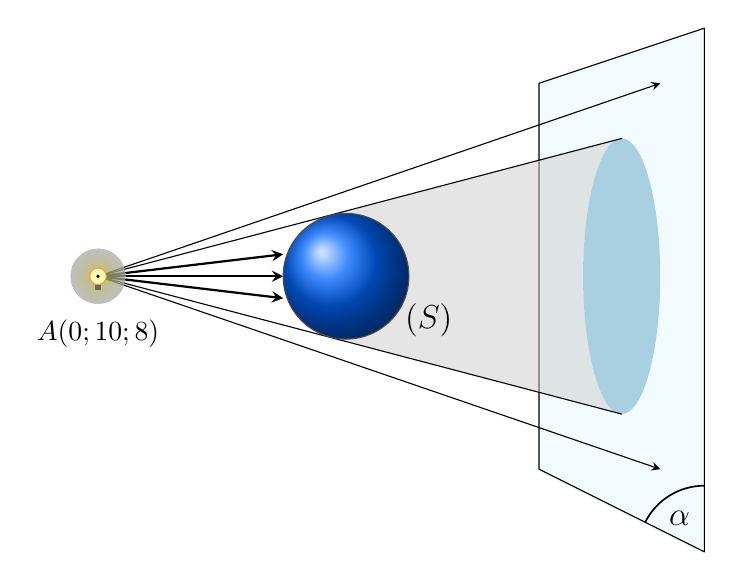
\begin{tikzpicture}[scale=0.7,>=stealth,line join=round,line cap=round,every node/.style={font=\large},
			declare function={xA = 0; yA = 2; xS = 4.5; yS = 2; R = 1.14; xSh = 9.5; ySh = 2; aSh = 0.7; bSh = 2.5; Sh = 2.5; dxT = -0.29; dyT = 1.1; xP1 = 8; yP1b = -1.5; yP1t = 5.5; xP2 = 11; yP2b = -3; yP2t =6.5; angleBot = 153.43; }]
			%%Mặt phẳng
			\draw[fill=cyan!5!white] (xP1,yP1t) -- (xP1,yP1b) -- (xP2,yP2b) -- (xP2,yP2t) -- cycle;
			\draw[line width=0.6pt] (xP2,yP2b+1.2) arc (90:angleBot:1.2);
			\node at (xP2-0.45,yP2b+0.6) {$\alpha$};
			%% Bóng của MC
			\fill[black!30!cyan,opacity=0.4] (xSh,ySh) ellipse (aSh and bSh);
			%%Vùng tối bên trong
			\fill[gray!40,opacity=0.5] (xS+dxT,yS+dyT) -- (xSh,ySh+bSh) arc (90:270:aSh and bSh) -- (xS+dxT,yS-dyT) -- cycle;
			%%hai tia sáng tiếp xúc MC
			\draw (xA,yA) -- (xSh,ySh+bSh);
			\draw (xA,yA) -- (xSh,ySh-bSh);
			%%hai tia sáng bên ngoài
			\draw[->] (xA,yA) -- (10.2,5.5);
			\draw[->] (xA,yA) -- (10.2,-1.5);
			%%3 mũi tên
			\draw[thick,->] (xA,yA) -- (xS-R,yS);
			\draw[thick,->] (xA,yA) -- (xS-R,yS+0.35*R);
			\draw[thick,->] (xA,yA) -- (xS-R,yS-0.35*R);
			%%Cầu
			\shade[ball color=blue!60!cyan] (xS,yS) circle (R);
			\draw[black!70] (xS,yS) circle (R);
			\node at (xS+1.5,yS-0.8) {$(S)$};
			%%Đèn
			\fill[inner color=yellow!60,outer color=white,opacity=0.5] (xA,yA) circle (0.5);
			\fill[yellow!30] (xA,yA) circle (0.15);
			\draw[orange!80] (xA,yA) circle (0.15);
			\fill[black!60] (xA-0.06,yA-0.15) rectangle (xA+0.06,yA-0.25);
			\draw[fill=black] (xA,yA) circle (0.6pt) node[font=\normalsize,below=12pt] {$A (0; 10; 8)$};
		\end{tikzpicture}
	}
	\choiceTF[t]
	{\True Mặt cầu $(S)$ có tâm $I(0;6;8)$, bán kính $R=2$}
	{\True Đường thẳng $AI$ có phương trình tham số là $\heva{&x=0\\&y=6+t\\&z=8}$}
	{\True Từ $A$ ta kẻ hai đường thẳng tiếp xúc với $(S)$ tại $M$ và $N$. Góc $\widehat{MAN}$ lớn nhất bằng $60^\circ$}
	{Bóng của $(S)$ trên mặt phẳng $(\alpha)$ là hình tròn có diện tích bằng $108\sqrt{3}\pi$}
	\loigiai{
		\begin{center}
			\begin{tikzpicture}[scale=.7,>=stealth,line join=round,line cap=round,every node/.style={font=\scriptsize},declare function={
					d = 9;
					phi = 30;
					xI = 5;
					Rs = (d-xI)*sin(phi);
					Rprime = d*tan(phi);
					Rxlarge = 0.7;
					Mx = xI + Rs*sin(phi);
					My = Rs*cos(phi);
					Rxsmall = 0.3;
				}]
				\path (0,0) coordinate (H);
				\path (xI,0) coordinate (I);
				\path (d,0) coordinate (A);
				\path (Mx,0) coordinate (K);
				\path (Mx,My) coordinate (M);
				\path (Mx,-My) coordinate (N);
				\path (0,Rprime) coordinate (Ttop);
				\path (0,-Rprime) coordinate (Tbot);
				\path (0,{-Rprime - 0.8}) coordinate (AlphaBot);
				\path (0,{Rprime + 0.8}) coordinate (AlphaTop);
				\fill[cyan!8] (0,0) ellipse ({Rxlarge} and {Rprime});
				\draw[line width=0.6pt] (AlphaBot) -- (AlphaTop);
				\draw[red!50!black,line width=0.6pt,dash pattern=on 2pt off 1.5pt] plot[domain=-90:90,samples=100] ({Rxlarge*cos(\x)},{Rprime*sin(\x)});
				\draw[red!50!black,line width=0.6pt] plot[domain=90:270,samples=100] ({Rxlarge*cos(\x)},{Rprime*sin(\x)});
				\draw[line width=0.6pt] (Ttop) -- (A) -- (Tbot);
				\draw[dashed,line width=0.6pt] (H) -- (A);
				\draw[line width=0.6pt] (I) circle (Rs);
				\draw[red!50!black,line width=0.6pt,dash pattern=on 2pt off 1.5pt] plot[domain=-90:90,samples=100] ({Mx + Rxsmall*cos(\x)},{My*sin(\x)});
				\draw[red!50!black,line width=0.6pt] plot[domain=90:270,samples=100] ({Mx + Rxsmall*cos(\x)},{My*sin(\x)});
				\draw[dashed,line width=0.6pt] (I) -- (M);
				\draw[line width=0.6pt] ($(A) + (180-phi:0.9)$) arc (180-phi:180:0.9);
				\node at ($(A) + ({180-phi/2}:1.2)$) {$\varphi$};
				\foreach \p/\pos in {H/180,I/-90,M/70,N/-70}{
					\draw (\p) circle (0.6pt) node[shift={(\pos:10pt)}] {$\p$};
				}
				\draw (K) circle (0.6pt);
				\draw (A) circle (0.6pt) node[anchor=west,shift={(2pt,0)}] {$A (0; 10; 8)$};
				\node[left] at ({-Rxlarge - 0.1},{Rprime/2}) {$(C')$};
				\node[left] at ({xI - Rs - 0.2},-0.8) {$(S)$};
				\node[right] at (0.1,{Rprime/2}) {$R'$};
				\node[right] at (AlphaBot) {$(\alpha)$};
			\end{tikzpicture}
		\end{center}
		\begin{itemchoice}
			\itemch 
			Mặt cầu $(S)\colon x^2+y^2+z^2-12y-16z+96=0$ có các hệ số $a=0$, $b=6$, $c=8$, $d=96$.\\
			Suy ra tâm mặt cầu là $I(0;6;8)$ và bán kính $R=\sqrt{0^2+6^2+8^2-96}=\sqrt{4}=2$.
			\itemch 
			Ta có $\overrightarrow{IA}=(0;4;0)=4(0;1;0)$.\\
			Đường thẳng $AI$ đi qua $I(0;6;8)$ và nhận vectơ $\overrightarrow{u}=(0;1;0)$ làm một vectơ chỉ phương.\\
			Do đó, phương trình tham số của đường thẳng $AI$ là $\heva{&x=0\\&y=6+t\\&z=8.}$		
			\immini{
				\itemch 
				Tập hợp các tiếp điểm của các tiếp tuyến kẻ từ điểm $A$ đến mặt cầu $(S)$ tạo thành một đường tròn nằm trên mặt cầu.\\
				Góc $\widehat{MAN}$ đạt giá trị lớn nhất khi và chỉ khi hai tiếp tuyến $AM$, $AN$ nằm trên hai đường sinh đối diện của hình nón ngoại tiếp mặt cầu $(S)$ đỉnh $A$.\\
				Xét tam giác $AMI$ vuông tại $M$ (do $AM$ là tiếp tuyến của $(S)$), ta có khoảng cách
				\[IA=\sqrt{0^2+(10-6)^2+0^2}=4.\]
				Khi đó $\sin\widehat{MAI}=\dfrac{IM}{IA}=\dfrac{R}{IA}=\dfrac{2}{4}=\dfrac{1}{2} \Rightarrow \widehat{MAI}=30^\circ.$\\
				Vậy góc lớn nhất $\widehat{MAN}=2\widehat{MAI}=60^\circ$.
			}{
				\begin{tikzpicture}[scale=0.55,>=stealth,line join=round,font=\footnotesize,line cap=round,declare function={r3=sqrt(3);}]
					\path
					(10,0) coordinate (A)
					(6,0) coordinate (I)
					(7,{r3}) coordinate (M)
					(7,{-r3}) coordinate (N)
					(1,{3*r3}) coordinate (P)
					(1,{-3*r3}) coordinate (Q)
					(1,0) coordinate (H);
					\draw[line width=1.2pt,cyan] (1,-6.5) -- (1,6.5) node[above right] {$(\alpha)$};
					\draw[line width=2pt,red] (P) -- (Q);
					\node[red,left] at (1,-4.5) {Bóng của $(S)$};
					\draw[thick,fill=blue!10] (I) circle (2);
					\draw[thick,orange] (A) -- (P);
					\draw[thick,orange] (A) -- (Q);
					\draw[dashed] (A) -- (H);
					\draw[dashed] (I) -- (M);
					\draw[dashed] (I) -- (N);
					\fill (A) circle (1.5pt) node[right] {$A$};
					\fill (I) circle (1.5pt) node[below left] {$I$};
					\fill (M) circle (1.5pt) node[above right] {$M$};
					\fill (N) circle (1.5pt) node[below right] {$N$};
					\draw (6.85,1.472) -- (7.11,1.322) -- (7.26,1.582);
					\draw (6.85,-1.472) -- (7.11,-1.322) -- (7.26,-1.582); 
					\draw (1.3,0) -- (1.3,0.3) -- (1,0.3); 
					\draw (9,0) arc (180:150:1);
					\node[rotate=60] at (6.2,0.9) {$R=2$};
				\end{tikzpicture}
			}
			\itemch 
			Bóng của quả cầu $(S)$ trên mặt phẳng $(\alpha)$ là một thiết diện được tạo bởi hình nón chiếu sáng (có đỉnh $A$, trục là đường thẳng $AI$, góc ở đỉnh $60^\circ$) cắt bởi mặt phẳng $(\alpha)\colon y-1=0$.\\
			Do đường thẳng $AI$ vuông góc với mặt phẳng $(\alpha)$ (vì vectơ chỉ phương $\overrightarrow{u}=(0;1;0)$ của $AI$ cùng phương với vectơ pháp tuyến $\overrightarrow{n}=(0;1;0)$ của $\alpha$), thiết diện bóng thu được là một hình tròn.\\
			Khoảng cách từ đỉnh nón $A(0;10;8)$ đến mặt phẳng $(\alpha)$ là
			\[h=\mathrm{d}\big(A,(\alpha)\big)=\dfrac{|10-1|}{\sqrt{0^2+1^2+0^2}}=9.\]
			Bán kính của hình tròn bóng (với thiết diện cắt ngang vuông góc trục) là 
			\[r=h \cdot \tan 30^\circ=9 \cdot \dfrac{1}{\sqrt{3}}=3\sqrt{3}.\]
			Diện tích của hình tròn bóng trên tường là 
			\[S=\pi r^2=\pi\left(3\sqrt{3}\right)^2=27\pi.\]
		\end{itemchoice}
	}
\end{ex}
%%%=============================%%%
\Closesolutionfile{ans}

\caukq
\Opensolutionfile{ans}[ans/ansTN-DienKhuyet]
%%%=============EX_17=============%%%
\begin{ex}%[1H8V5-4]%[TDMZD03]%[Võ Hiệp]
	Cho hình chóp cụt tứ giác đều $ABCD.A'B'C'D'$ có độ dài các cạnh $AB=8$, $A'B'=4$, $AA'=6$. Hãy tính khoảng cách giữa hai đường thẳng $AA'$ và $CD$ ({\it làm tròn kết quả đến hàng phần mười}).
	\par
	\shortans[0]{7,5}
	\loigiai{
		\immini{
			Kéo dài $4$ cạnh bên đồng quy tại điểm $S$, ta có $S.ABCD$ là hình chóp tứ giác đều.\\
			Xét tam giác $SAB$ có $A'B' \parallel AB$, theo định lí Thalès ta có
			\[\dfrac{SA'}{SA}=\dfrac{A'B'}{AB}=\dfrac{4}{8}=\dfrac{1}{2} \Rightarrow SA=2SA'.\]
			Lại có $SA - SA' = AA' = 6 \Rightarrow 2SA' - SA' = 6 \Rightarrow SA' = 6$.\\
			Do đó $SA=12$.\\
			Gọi $O$ là giao điểm của $AC$ và $BD$. Vì $ABCD$ là hình vuông cạnh bằng $8$ nên $AC=BD=8\sqrt{2}$.\\
			Suy ra $OA=OB=OC=OD=4\sqrt{2}$.\\
			Vì $S.ABCD$ là hình chóp tứ giác đều nên $SO \perp (ABCD)$.
		}{
			\begin{tikzpicture}[font=\scriptsize,line join=round,line cap=round,>=stealth]
				\tikzset{declare function={a=4.5; b=2.2; h=4.5;}}
				\path (0,0) coordinate (A)
				(a,0) coordinate (D)
				(-150:b) coordinate (B)
				($(B)+(D)$) coordinate (C)
				($(A)!0.5!(C)$) coordinate (O)
				($(O)+(0,h)$) coordinate (S)
				($(S)!0.5!(A)$) coordinate (A')
				($(S)!0.5!(B)$) coordinate (B')
				($(S)!0.5!(C)$) coordinate (C')
				($(S)!0.5!(D)$) coordinate (D')
				($(A)!0.5!(B)$) coordinate (M)
				($(S)!(O)!(M)$) coordinate (H);
				\foreach \x/\y/\z in {A/O/S,D/O/S,A/M/O,O/H/M}{
					\path (\y) pic[draw,angle radius=5pt]{right angle = \x--\y--\z};
				}
				\draw[dashed] (B)--(A)--(D)
				(A)--(C)
				(B)--(D)
				(S)--(A)
				(S)--(O)
				(B')--(A')--(D')
				(S)--(M)
				(O)--(M)
				(O)--(H);
				\draw (S)--(B)--(C)--(D)--cycle (S)--(C)
				(B')--(C')--(D');
				\foreach \t/\g in {A/-90,B/-90,C/-60,D/60,S/90,O/-90,A'/-50,B'/180,C'/0,D'/60,M/-90,H/180}{
					\fill (\t) circle (1pt) node[shift={(\g:7pt)},font=\scriptsize]{$\t$};
				}
			\end{tikzpicture}
		}
		\noindent
		Trong tam giác vuông $SOA$ tại $O$, ta có
		\[SO=\sqrt{SA^2-OA^2}=\sqrt{12^2-\left(4\sqrt{2}\right)^2}=4\sqrt{7}.\]
		Ta có $AA' \subset SA$, suy ra $\mathrm{d}(AA', CD) = \mathrm{d}(SA, CD)$.\\
		Vì $CD \parallel AB$ và $AB \subset (SAB)$ nên $CD \parallel (SAB)$.\\
		Suy ra $\mathrm{d}(SA, CD) = \mathrm{d}\big(CD, (SAB)\big) = \mathrm{d}\big(C, (SAB)\big)$.\\
		Mặt khác, $CO \cap (SAB) = A$ nên
		\[\dfrac{\mathrm{d}\big(C, (SAB)\big)}{\mathrm{d}\big(O, (SAB)\big)} = \dfrac{CA}{OA} = 2 \Rightarrow \mathrm{d}\big(C, (SAB)\big) = 2\mathrm{d}\big(O, (SAB)\big).\]
		Kẻ $OM \perp AB$ tại $M$, kẻ $OH \perp SM$ tại $H$.\\
		Ta có $\heva{&AB \perp OM\\&AB \perp SO} \Rightarrow AB \perp (SOM) \Rightarrow AB \perp OH$.\\
		Mà $OH \perp SM$, suy ra $OH \perp (SAB)$.\\
		Do đó $\mathrm{d}\big(O, (SAB)\big) = OH$.\\
		Vì $ABCD$ là hình vuông tâm $O$ nên $OM = \dfrac{1}{2}BC = 4$.\\
		Xét tam giác $SOM$ vuông tại $O$, có đường cao $OH$, ta có
		\[\dfrac{1}{OH^2} = \dfrac{1}{SO^2} + \dfrac{1}{OM^2} \Rightarrow OH = \dfrac{SO \cdot OM}{\sqrt{SO^2 + OM^2}} = \dfrac{4\sqrt{7} \cdot 4}{\sqrt{\left(4\sqrt{7}\right)^2 + 4^2}} = \sqrt{14}.\]
		Suy ra $\mathrm{d}\big(C, (SAB)\big) = 2\sqrt{14}$.\\
		Vậy khoảng cách giữa hai đường thẳng $AA'$ và $CD$ là $2\sqrt{14} \approx 7{,}5$.
	}
\end{ex}
%%%=============================%%%

%%%=============EX_18=============%%%
\begin{ex}%[2D1H3-6]%[TDMZD03]%[Duong Xuan Loi]
	Một công ty sản xuất một loại sản phẩm với chi phí để sản xuất một sản phẩm là $400$ nghìn đồng và bán ra mỗi sản phẩm là $600$ nghìn đồng. Biết rằng số lượng sản phẩm bán ra tăng theo số tiền chi cho quảng cáo là $n(x)=A+B\sqrt{x+100}$ (sản phẩm), trong đó $x$ là số tiền chi cho quảng cáo tính theo đơn vị triệu đồng. Khi không chi cho quảng cáo thì bán được $700$ sản phẩm, khi chi $21$ triệu đồng thì bán được $760$ sản phẩm. Hãy tính theo đơn vị triệu đồng lợi nhuận lớn nhất thu được (\textit{làm tròn kết quả đến hàng đơn vị}).
	\par
	\shortans[0]{140}
	\loigiai{
		Theo bài ra, ta có hệ phương trình
		\[\heva{& n(0)=700 \\ & n(21)=760} \Leftrightarrow \heva{& A+B\sqrt{100}=700 \\ & A+B\sqrt{121}=760} \Leftrightarrow \heva{& A+10B=700 \\ & A+11B=760} \Leftrightarrow \heva{& A=100 \\ & B=60.}\]
		Suy ra hàm số biểu thị số lượng sản phẩm bán ra là $n(x)=100+60\sqrt{x+100}$.\\		
		Mỗi sản phẩm bán được mang lại số tiền lãi là 
		\[600 - 400 = 200 \text{ (nghìn đồng)} = 0{,}2 \text{ (triệu đồng)}.\]
		Hàm số biểu thị lợi nhuận thu được (đơn vị triệu đồng) theo số tiền chi cho quảng cáo $x$ (với $x \ge 0$) là
		\[P(x)=0{,}2n(x)-x=0{,}2\left(100+60\sqrt{x+100}\right)-x=20+12\sqrt{x+100}-x.\]
		Đạo hàm của hàm số lợi nhuận là
		\[P'(x)=12 \cdot \dfrac{1}{2\sqrt{x+100}}-1=\dfrac{6}{\sqrt{x+100}}-1.\]
		Xét phương trình $P'(x)=0$
		\[\dfrac{6}{\sqrt{x+100}}-1=0 \Leftrightarrow \sqrt{x+100}=6 \Leftrightarrow x+100=36 \Leftrightarrow x=-64 \text{ (loại vì } x \ge 0).\]
		Ta thấy với mọi $x \ge 0$, ta có $\sqrt{x+100} \ge 10 \Rightarrow \dfrac{6}{\sqrt{x+100}} \le \dfrac{6}{10} < 1$.\\
		Do đó $P'(x) < 0$ với mọi $x \ge 0$.\\
		Suy ra hàm số $P(x)$ luôn nghịch biến trên nửa khoảng $[0; +\infty)$.\\
		Bảng biến thiên
		\begin{center}
			
\begin{tikzpicture}
				\tkzTabInit[nocadre=false, lgt=1.2, espcl=3, deltacl=0.5]
				{$x$ /0.7, $P'(x)$ /0.7, $P(x)$ /2}
				{$0$,$+\infty$}
				\tkzTabLine{,-,}
				\tkzTabVar{+/$140$, -/$-\infty$}
			\end{tikzpicture}
		\end{center}		
		Từ bảng biến thiên, ta thấy $\max\limits_{[0; +\infty)} P(x) = P(0) = 140$.\\
		Vậy lợi nhuận lớn nhất công ty thu được là $140$ triệu đồng (đạt được khi không chi tiền quảng cáo).
	}
\end{ex}
%%%=============================%%%

%%%=============EX_19=============%%%
\begin{ex}%[0D0V2-6]%[TDMZD03]%[Lê Hồ Quang Minh]
	Cho hình đa giác đều $(H)$ gồm có $26$ đỉnh. Chọn ngẫu nhiên $5$ đỉnh của $(H)$. Hãy tính xác suất để chọn được một ngũ giác mà không có cạnh nào là cạnh của $(H)$ \textit{(làm tròn kết quả đến hàng phần trăm)}?
	\par
	\shortans[0]{0,38}
	\loigiai{
		Số phần tử của không gian mẫu là $n(\Omega) = \mathrm{C}_{26}^5 = 65\,780$.\\
		\immini{
			Chọn một đỉnh $A$ và một ngũ giác như hình vẽ. Gọi số cạnh trên các cung lần lượt là $x_1$, $x_2$, $x_3$, $x_4$, $x_5$. Để các cạnh của ngũ giác không phải là cạnh của đa giác thì số cạnh trên mỗi cung phải lớn hơn $1$ (tức là lớn hơn hoặc bằng $2$) và tất nhiên tổng số cạnh trên các cung phải bằng $26$. Khi đó ta có
			\[ \heva{& x_1, x_2, x_3, x_4, x_5 \ge 2 \\ & x_1+x_2+x_3+x_4+x_5 = 26.} \]
		}{
			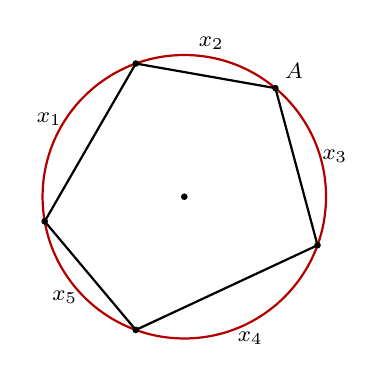
\begin{tikzpicture}[scale=1.2, font=\footnotesize, line join=round, line cap=round, >=stealth]
				\coordinate (O) at (0,0);
				\draw[thick, red!70!black] (O) circle (1.5);
				\fill (O) circle (1pt);
				\coordinate (A) at (50:1.5);
				\coordinate (P1) at (110:1.5);
				\coordinate (P2) at (190:1.5);
				\coordinate (P3) at (250:1.5);
				\coordinate (P4) at (340:1.5);
				\draw[thick] (A) -- (P1) -- (P2) -- (P3) -- (P4) -- cycle;
				\fill (A) circle (1pt) node[above right] {$A$};
				\fill (P1) circle (1pt);
				\fill (P2) circle (1pt);
				\fill (P3) circle (1pt);
				\fill (P4) circle (1pt);
				\node at (80:1.65) {$x_2$};
				\node at (150:1.65) {$x_1$};
				\node at (220:1.65) {$x_5$};
				\node at (295:1.65) {$x_4$};
				\node at (15:1.65) {$x_3$};
			\end{tikzpicture}
		}
		\noindent
		Chúng ta đưa về chuẩn phương trình nghiệm nguyên dương Euler như sau
		\[ \heva{& (x_1-1), (x_2-1), (x_3-1), (x_4-1), (x_5-1) \ge 1 \\ & (x_1-1) + (x_2-1) + (x_3-1) + (x_4-1) + (x_5-1) = 26-5=21.} \]
		Đặt $X_1 = x_1-1$, $X_2 = x_2-1$, $X_3 = x_3-1$, $X_4 = x_4-1$, $X_5 = x_5-1$, suy ra
		\begin{align*}
			\heva{& X_1, X_2, X_3, X_4, X_5 \ge 1 \\ & X_1+X_2+X_3+X_4+X_5 = 21.} \tag{*}
		\end{align*}
		Rõ ràng ứng với mỗi bộ $(X_1; X_2; X_3; X_4; X_5)$ cho ta một bộ $(x_1; x_2; x_3; x_4; x_5)$, cũng chính là một ngũ giác thỏa mãn bài toán. Suy ra số ngũ giác thỏa mãn bài toán bằng số nghiệm nguyên dương $(X_1; X_2; X_3; X_4; X_5)$ của $(*)$ và bằng số cách chia $21$ chiếc kẹo giống nhau cho $5$ em bé sao cho mỗi em bé được ít nhất một chiếc kẹo và bằng $\mathrm{C}_{21-1}^{5-1} = \mathrm{C}_{20}^4$.\\
		Ta làm việc với $26$ đỉnh và nhớ rằng quá trình đếm nó bị lặp $5$ lần (mỗi ngũ giác có $5$ đỉnh vai trò như nhau, mỗi khi ta chọn tới một đỉnh của ngũ giác đó thì nó sẽ bị lặp $1$ lần), cho nên ta suy ra số ngũ giác thỏa mãn bài toán là
		\[ T = \dfrac{26 \cdot \mathrm{C}_{20}^4}{5} = 25\,194. \]
		Suy ra xác suất cần tìm là
		\[ \mathrm{P} = \dfrac{25\,194}{\mathrm{C}_{26}^5} \approx 0{,}38. \]
	}
\end{ex}
%%%=============================%%%

%%%=============EX_20=============%%%
\begin{ex}%[2D4V3-2]%[TDMZD03]%[Nguyễn Đức Tuấn Anh]
	Hình vẽ số $2$ bên phải mô tả phần diện tích cần tô màu. Biết rằng $4$ tâm của $4$ đường tròn tạo thành hình vuông $ABCD$ có cạnh bằng $20$ cm, bán kính đường tròn tâm $A$ bằng $20$ cm, các đường tròn tâm $B$ và $D$ có cùng bán kính bằng $6$ cm và tiếp xúc ngoài với đường tròn tâm $C$. Hãy tính theo đơn vị centimet vuông diện tích phần hình phẳng cần tô màu (\textit{làm tròn kết quả đến hàng đơn vị}).
	\begin{center}
		\begin{tikzpicture}[scale=.6, font=\footnotesize, line join=round, line cap=round, >=stealth]
			\begin{scope}[shift={(-5.5, 0)}]
				\coordinate (A) at (0,0);
				\coordinate (B) at (45:4);
				\coordinate (C) at (0, {4*sqrt(2)});
				\coordinate (D) at (135:4);
				\draw[fill=white, line width=1pt] (0,0) circle (4);
				\begin{scope}
					\clip (0,0) circle (4);
					\draw[line width=7pt] (-4, 0.0) .. controls (-1.5, -1.0) and (1.5, -1.0) .. (4, 0.0);
					\draw[line width=1pt] (-4, 0.5) .. controls (-1.5, -0.5) and (1.5, -0.5) .. (4, 0.5);
					\draw[line width=1pt] (-4, -0.5) .. controls (-1.5, -1.5) and (1.5, -1.5) .. (4, -0.5);
				\end{scope}
				\draw[fill=white, line width=1pt] (0, 0.8) circle (0.45);
				\draw[fill=white, line width=1pt] (0, -0.9) circle (0.45);
				\draw[fill=white, line width=1pt] (0, -2.6) circle (0.45);
				\draw[fill=white, line width=1pt] (B) circle (1.2);
				\draw[fill=white, line width=1pt] (D) circle (1.2);
				\draw[fill=white, line width=1pt] (C) circle (2.8);
				\draw[fill=white, line width=1pt] (C) circle (2.2);
				\begin{scope}[shift={(90:0.5)}]
					\clip (C) circle (2.2);
					\draw[line width=1.2pt] (-2.5, 5.8) .. controls (-1.6, 5.4) .. (-1.0, 5.6) -- (-0.8, 6.2) .. controls (-0.4, 5.4) .. (0.1, 5.6) -- (0.3, 6.1) .. controls (0.7, 5.4) .. (1.2, 5.5) -- (1.5, 6.0) .. controls (1.8, 5.5) .. (2.5, 5.4);
					\draw[line width=1pt] (-0.15, 4.2) .. controls (0, 4.1) and (0, 4.1) .. (0.15, 4.2);
					\fill[black] (-0.35, 3.8) .. controls (-0.15, 3.7) and (0.15, 3.7) .. (0.35, 3.8) .. controls (0.25, 3.3) and (-0.25, 3.3) .. cycle;
					\begin{scope}[shift={(-0.8, 5.0)}]
						\draw[line width=1.5pt] (-0.4, 0.3) .. controls (-0.1, 0.6) and (0.3, 0.5) .. (0.5, 0.2);
						\fill[black] (0.05, 0) ellipse (0.25 and 0.35);
						\fill[white] (-0.05, 0.15) ellipse (0.08 and 0.12);
						\fill[white] (0.15, -0.15) circle (0.06);
						\draw[line width=.75pt] (-0.2, -0.3) .. controls (0, -0.4) and (0.2, -0.3) .. (0.3, -0.2);
					\end{scope}
					\begin{scope}[shift={(0.8, 5.0)}, xscale=-1]
						\draw[line width=1.5pt] (-0.4, 0.3) .. controls (-0.1, 0.6) and (0.3, 0.5) .. (0.5, 0.2);
						\fill[black] (0.05, 0) ellipse (0.25 and 0.35);
						\fill[white] (-0.05, 0.15) ellipse (0.08 and 0.12);
						\fill[white] (0.15, -0.15) circle (0.06);
						\draw[line width=.75pt] (-0.2, -0.3) .. controls (0, -0.4) and (0.2, -0.3) .. (0.3, -0.2);
					\end{scope}
				\end{scope}
				\node[red!80!black] at (0, -5) {Hình $1$};
			\end{scope}
			\draw[cyan, thick, rounded corners=1pt] (-1.2, 2.7) -- (0.3, 2.7) -- (0.3, 3.0) -- (1.5, 2.5) -- (0.3, 2.0) -- (0.3, 2.3) -- (-1.2, 2.3) -- cycle;
			\begin{scope}[shift={(6.5, -0.5)}]
				\coordinate (A) at (0,0);
				\coordinate (B) at (45:4);
				\coordinate (C) at (0, {4*sqrt(2)});
				\coordinate (D) at (135:4);
				\draw[line width=1pt,fill=cyan!10] (A) circle (4);
				\draw[line width=1pt,fill=cyan!10] (B) circle (1.2);
				\draw[line width=1pt,fill=cyan!10] (C) circle (2.8);
				\draw[line width=1pt,fill=cyan!10] (D) circle (1.2);
				\draw[cyan, thick] (A) -- (B) -- (C) -- (D) -- cycle;
				\fill[red!80!black] (A) circle (2pt) node[below=2pt] {$A$};
				\fill[red!80!black] (B) circle (2pt) node[right=2pt] {$B$};
				\fill[red!80!black] (C) circle (2pt) node[above=2pt] {$C$};
				\fill[red!80!black] (D) circle (2pt) node[left=2pt] {$D$};
				\pic[draw, angle radius=2mm] {right angle = B--A--D};
				\node[red!80!black] at (0, -5.0) {Hình $2$};
			\end{scope}
		\end{tikzpicture}
	\end{center}
	\par
	\shortans[0]{1921}
	\loigiai{
		\textbf{Cách 1: Tính diện tích bằng hình học lượng giác}\\
		\immini{
			Ta có $ABCD$ là hình vuông cạnh $20$\,cm nên $BC=CD=20$\,cm.\\
			Đường tròn tâm $B$ tiếp xúc ngoài với đường tròn tâm $C$ nên $R_B + R_C = BC \Leftrightarrow 6 + R_C = 20 \Rightarrow R_C = 14$\,cm.\\
			Gọi $P_B$ là giao điểm nằm ngoài hình vuông $ABCD$ của hai đường tròn tâm $A$ và tâm $B$.\\
			Tương tự, gọi $P_D$ là giao điểm nằm ngoài hình vuông $ABCD$ của hai đường tròn tâm $A$ và tâm $D$.\\
			Xét $\triangle A B P_B$, ta có $AB=20$\,cm, $AP_B=20$\,cm, $BP_B=6$\,cm.\\
			Đặt $\alpha = \widehat{ABP_B}$ và $\beta = \widehat{BAP_B}$.\\
			Áp dụng định lí cosin trong $\triangle A B P_B$, ta có
			\[ \cos \alpha = \dfrac{AB^2+BP_B^2-AP_B^2}{2 \cdot AB \cdot BP_B} = \dfrac{20^2+6^2-20^2}{2 \cdot 20 \cdot 6} = 0{,}15 \Rightarrow \alpha \approx 1{,}4202 \text{ rad}. \]
		}{
			\begin{tikzpicture}[scale=.7, font=\footnotesize, line join=round, line cap=round, >=stealth]
				\coordinate (A) at (0,0);
				\coordinate (B) at (45:4);
				\coordinate (C) at (0, {4*sqrt(2)});
				\coordinate (D) at (135:4);
				\pic[draw, angle radius=2mm] {right angle = B--A--D};
				\draw[] (A) circle (4);
				\draw[fill=white] (B) circle (1.2);
				\draw[fill=white] (C) circle (2.8);
				\draw[fill=white] (D) circle (1.2);
				\draw[] (A) -- (B) -- (C) -- (D) -- cycle;
				\pgfmathsetmacro{\betaAngle}{acos((4^2 + 4^2 - 1.2^2) / (2 * 4 * 4))}
				\coordinate (PB) at ({45-\betaAngle}:4);
				\coordinate (PD) at ({135+\betaAngle}:4);
				\draw[] (A) -- (PB) -- (B);
				\draw[] (A) -- (PD) -- (D);
				\pic[draw, "$\beta$", angle radius=10mm,double, angle eccentricity=1.2, font=\footnotesize] {angle = PB--A--B};
				\pic[draw, "$\alpha$", angle radius=3mm, angle eccentricity=1.5, font=\footnotesize] {angle = A--B--PB};
				
				\pic[draw, "$\beta$", angle radius=10mm,double, angle eccentricity=1.2, font=\footnotesize] {angle = D--A--PD};
				\pic[draw, "$\alpha$", angle radius=3mm, angle eccentricity=1.5, font=\footnotesize] {angle = PD--D--A};
				\fill[red!80!black] (A) circle (1.5pt) node[below] {$A$};
				\fill[red!80!black] (B) circle (1.5pt) node[right] {$B$};
				\fill[red!80!black] (C) circle (1.5pt) node[above] {$C$};
				\fill[red!80!black] (D) circle (1.5pt) node[left] {$D$};
				\fill[] (PB) circle (1.5pt) node[right] {$P_B$};
				\fill[] (PD) circle (1.5pt) node[left] {$P_D$};
			\end{tikzpicture}
		}
		\noindent Do $\triangle A B P_B$ cân tại $A$ (vì $AB=AP_B=20$) nên $\widehat{AP_BB} = \widehat{ABP_B} = \alpha$, suy ra $\beta = \pi - 2\alpha$.\\
		Diện tích $\triangle A B P_B$ là $S_{\triangle A B P_B} = \dfrac{1}{2} \cdot AB \cdot BP_B \cdot \sin \alpha = \dfrac{1}{2} \cdot 20 \cdot 6 \cdot \sqrt{1 - 0{,}15^2} = 3\sqrt{391}$ (cm$^2$).\\
		Diện tích phần hình phẳng cần tô màu bằng tổng diện tích đa giác $C B P_B A P_D D$ (được tạo thành từ hình vuông $ABCD$ và hai tam giác $A B P_B$, $A D P_D$) và $4$ hình quạt tròn nằm ngoài đa giác này.\\
		Diện tích đa giác là $S_{\text{đg}} = S_{ABCD} + 2S_{\triangle A B P_B} = 400 + 6\sqrt{391}\,\left(\text{cm}^2\right)$.\\
		Diện tích $4$ hình quạt tròn nằm ngoài đa giác gồm
		\begin{itemize}
			\item Hình quạt tâm $C$ có góc ở tâm $360^\circ - 90^\circ = 270^\circ$, diện tích $S_C = \dfrac{1}{2} \cdot 14^2 \cdot \dfrac{3\pi}{2} = 147\pi\,\left(\text{cm}^2\right)$.
			\item Hình quạt tâm $B$ có góc ở tâm $360^\circ - (90^\circ + \alpha) = 270^\circ - \alpha$, diện tích $S_B = \dfrac{1}{2} \cdot 6^2 \cdot \left(\dfrac{3\pi}{2} - \alpha\right) = 27\pi - 18\alpha\,\left(\text{cm}^2\right)$.
			\item Hình quạt tâm $D$ hoàn toàn tương tự, diện tích $S_D = 27\pi - 18\alpha\,\left(\text{cm}^2\right)$.
			\item Hình quạt tâm $A$ có góc ở tâm $360^\circ - (90^\circ + 2\beta) = 270^\circ - 2\beta$, diện tích $S_A = \dfrac{1}{2} \cdot 20^2 \cdot \left(\dfrac{3\pi}{2} - 2\beta\right) = 300\pi - 400\beta\,\left(\text{cm}^2\right)$.
		\end{itemize}
		Tổng diện tích $4$ hình quạt là
		\[ S_{\text{hq}} = 147\pi + 2(27\pi - 18\alpha) + 300\pi - 400\beta = 501\pi - 36\alpha - 400\beta\,\left(\text{cm}^2\right). \]
		Thay $\beta = \pi - 2\alpha$ vào biểu thức trên, ta được
		\[ S_{\text{hq}} = 501\pi - 36\alpha - 400(\pi - 2\alpha) = 101\pi + 764\alpha\,\left(\text{cm}^2\right). \]
		Tổng diện tích phần hình phẳng cần tô màu là
		\[ S = S_{\text{đg}} + S_{\text{hq}} = 400 + 6\sqrt{391} + 101\pi + 764\alpha \approx 1\,921 \,\left(\text{cm}^2\right). \]		
		\textbf{Cách 2: Tính diện tích bằng ứng dụng tích phân}\\
		\immini{
			Dễ thấy đường tròn tâm $C$ có bán kính là $R_C = BC - 6 = 20 - 6 = 14$\,(cm).\\
			Diện tích cần tô màu được tính bằng tổng của: diện tích hình vuông $ABCD$, $\dfrac{3}{4}$ diện tích hình tròn tâm $A$, $\dfrac{3}{4}$ diện tích hình tròn tâm $C$, $2$ nửa diện tích hình tròn tâm $B$, $2$ lần diện tích $S_1$.\\
			Để tính diện tích $S_1$, ta đi tính diện tích $S_2$ và có $S_1 = \dfrac{1}{4}\pi \cdot 6^2 - S_2$.\\
			Gắn hệ trục tọa độ $Oxy$ như hình vẽ (gốc $O \equiv B$, trục hoành $Ox$ chứa tia đối của tia $BC$, trục tung $Oy$ chứa tia đối của tia $BA$).\\
			Ta có phương trình đường tròn tâm $B$ là $x^2 + y^2 = 36 \Rightarrow$ phương trình của đoạn cung giới hạn nên $S_2$ là $y = -\sqrt{36 - x^2}$.\\
			Đường tròn tâm $A$ có tọa độ $A(0;-20)$ nên có phương trình là $x^2 + (y+20)^2 = 400 \Rightarrow$ phương trình của đoạn cung giới hạn nên $S_2$ là $y = -20 + \sqrt{400 - x^2}$.
		}{
			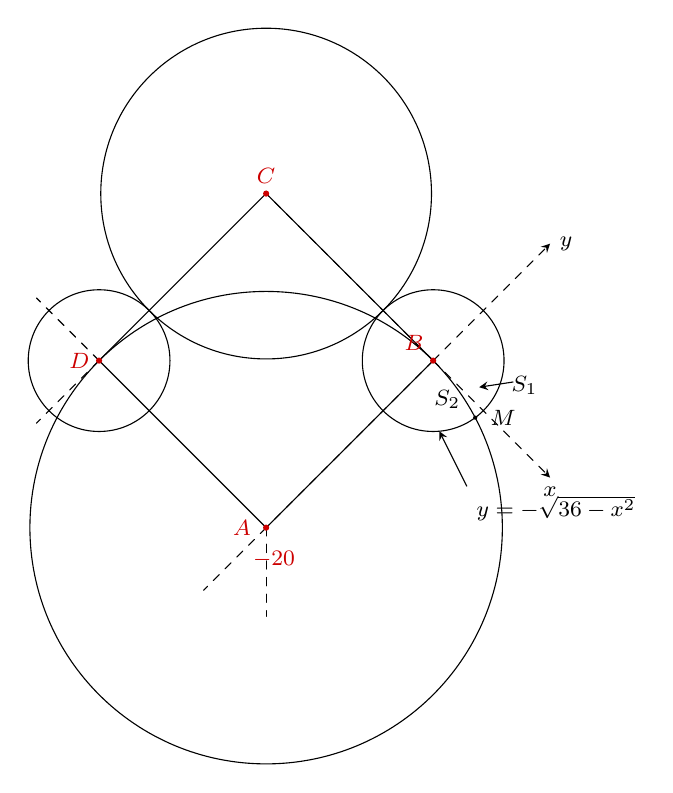
\begin{tikzpicture}[scale=.75, font=\footnotesize, line join=round, line cap=round, >=stealth]
				\coordinate (A) at (0,0);
				\coordinate (B) at (45:4);
				\coordinate (C) at (0, {4*sqrt(2)});
				\coordinate (D) at (135:4);
				\draw (A) circle (4);
				\draw (B) circle (1.2);
				\draw (C) circle (2.8);
				\draw (D) circle (1.2);
				\draw (A) -- (B) -- (C) -- (D) -- cycle;
				\draw[->, dashed] (B) -- ++(-45:2.8) node[below] {$x$};
				\draw[->, dashed] (B) -- ++(45:2.8) node[right] {$y$};
				\draw[dashed] (B) -- (A);
				\draw[dashed] (B) -- (C);
				\draw[dashed] (D) -- ++(225:1.5);
				\draw[dashed] (D) -- ++(135:1.5);
				\draw[dashed] (A) -- ++(-90:1.5);
				\draw[dashed] (A) -- ++(225:1.5);
				\fill[red!80!black] (A) circle (1.5pt) node[shift={(0.1,-0.4)}] {$-20$} node[left=2pt] {$A$};
				\fill[red!80!black] (B) circle (1.5pt) node[above left] {$B$};
				\fill[red!80!black] (C) circle (1.5pt) node[above] {$C$};
				\fill[red!80!black] (D) circle (1.5pt) node[left] {$D$};
				\coordinate (M) at ([shift={(-53.6:1.2)}]B);
				\fill (M) circle (1pt) node[right=2pt] {$M$};
				\node at ([shift={(-70:0.7)}]B) {$S_2$};
				\node at ([shift={(-15:1.6)}]B) {$S_1$};
				\draw[->] ([shift={(-15:1.4)}]B) -- ([shift={(-30:0.9)}]B);
				\node[below right] at ([shift={(-75:2.2)}]B) {$y=-\sqrt{36-x^2}$};
				\draw[->] ([shift={(-75:2.2)}]B) -- ([shift={(-85:1.2)}]B);
			\end{tikzpicture}
		}
		\noindent Hai đường tròn này cắt nhau tại điểm $M$ có tọa độ được xác định bởi hệ phương trình
		\[ \heva{& x^2 + y^2 = 36 \\ & x^2 + (y+20)^2 = 400 \\ & x > 0} \Rightarrow \heva{& y = -0{,}9 \\ & x = \dfrac{3\sqrt{391}}{10}.} \]
		Suy ra diện tích $S_2$ là
		\[ S_2 = \displaystyle\int\limits_0^{\frac{3\sqrt{391}}{10}} \left[ \left(-20 + \sqrt{400 - x^2}\right) - \left(-\sqrt{36 - x^2}\right) \right] \mathrm{d}x \approx 26{,}47\dots \]
		Vậy suy ra diện tích phần hình phẳng cần tô màu là
		\begin{align*}
			S &= 20^2 + \dfrac{3}{4}\pi \cdot 20^2 + \dfrac{3}{4}\pi \cdot 14^2 + 2 \cdot \dfrac{1}{2}\pi \cdot 6^2 + 2S_1 \\
			&= 20^2 + \dfrac{3}{4}\pi \cdot 20^2 + \dfrac{3}{4}\pi \cdot 14^2 + 2 \cdot \dfrac{1}{2}\pi \cdot 6^2 + 2 \left( \dfrac{1}{4}\pi \cdot 6^2 - S_2 \right) \\
			&= 20^2 + \dfrac{3}{4}\pi \cdot 20^2 + \dfrac{3}{4}\pi \cdot 14^2 + 2 \cdot \dfrac{1}{2}\pi \cdot 6^2 + 2 \left( \dfrac{1}{4}\pi \cdot 6^2 - 26{,}47\dots \right) \\
			&\approx 1\,921 \text{ (cm}^2).
		\end{align*}
	}
\end{ex}
%%%=============================%%%

%%%=============EX_21=============%%%
\begin{ex}%[2H5C2-8]%[TDM32]%[Nguyễn Văn Sang]
	Trong không gian $Oxyz$ đơn vị dài trên mỗi trục là mét, có hai chiếc gương thần kì có mặt phản xạ vào nhau, gương thứ nhất nằm trên mặt phẳng $(G_1) \colon z = 0$ và gương thứ hai nằm trên mặt phẳng $(G_2) \colon y + 2z - 4 = 0$. Ánh mắt của hoàng tử đặt tại $S(3; 0; 1{,}7)$ và ánh mắt của công chúa đặt tại $A(0; 5; 1{,}6)$. Hoàng tử phát ra một tia sáng $SM$ đến gặp một gương tại $M$, tại đây tia sáng bị bật trở lại và chiếc gương này biến mất, tia sáng gặp gương còn lại tại điểm $N$, tại $N$ tia sáng sẽ bị bật trở lại, tia sáng sẽ đến điểm $A$. Hoàng tử sẽ vượt qua được thử thách (để cưới được công chúa) nếu tổng $SM + MN + NA$ nhỏ nhất. Hãy xác định giá trị nhỏ nhất này theo đơn vị mét \textit{(làm tròn kết quả đến hàng phần mười)}.
	\par
	\shortans[0]{6,8}
	\loigiai{
%	\begin{center}
%			\begin{tikzpicture}[>=stealth,line join=round,line cap=round,every node/.style={font=\large}]
%			\tikzset{
%				declare function={
%					Xx = -3; Xy = -2.4;
%					Yx = 4.5; Yy = 0;
%					Zx = 0; Zy = 3;
%					Xux = -3; Xuy = 0.6;
%					Xyx = 1.5; Xyy = -2.4;
%					Spx = -0.4; Spy = 3.6;
%					Apx = 4.2; Apy = -2.2;
%					Sx = -2.0; Sy = 1.5;
%					Ax = 4.2; Ay = 2.2;
%					tM = 0.35;
%					Mx = Spx + tM*(Apx - Spx);
%					My = Spy + tM*(Apy - Spy);
%					tN = 0.75;
%					Nx = Spx + tN*(Apx - Spx);
%					Ny = Spy + tN*(Apy - Spy);
%				}
%			}
%			\coordinate (O) at (0,0);
%			\coordinate (X0) at (Xx,Xy);
%			\coordinate (Y0) at (Yx,Yy);
%			\coordinate (Z0) at (Zx,Zy);
%			\coordinate (Xu) at (Xux,Xuy);
%			\coordinate (Xy_c) at (Xyx,Xyy);
%			\coordinate (Sp) at (Spx,Spy);
%			\coordinate (Ap) at (Apx,Apy);
%			\coordinate (S) at (Sx,Sy);
%			\coordinate (A) at (Ax,Ay);
%			\coordinate (M) at (Mx,My);
%			\coordinate (N) at (Nx,Ny);
%			\draw[-Stealth,line width=0.7pt,red!70!black] (0,0) -- (-3.5,-2.8) node[left,text=black] {$x$};
%			\draw[-Stealth,line width=0.7pt,red!70!black] (0,0) -- (6,0) node[below,text=black] {$y$};
%			\draw[-Stealth,line width=0.7pt,red!70!black] (0,0) -- (0,4.5) node[right,text=black] {$z$};
%			\draw[line width=0.6pt] (X0) -- (Xu) -- (Z0);
%			\draw[line width=0.6pt] (Xu) -- (Xy_c);
%			\draw[line width=0.6pt] (X0) -- (Xy_c);
%			\draw[line width=0.6pt] (Xy_c) -- (Y0);
%			\draw[densely dotted,line width=0.6pt] (Z0) -- (Y0);
%			\draw[line width=0.6pt] (X0) ++(0:0.7) arc (0:38.6:0.7);
%			\node at (-1.9,-2.15) {$G_1$};
%			\draw[line width=0.6pt] (Xy_c) ++(146.3:0.7) arc (146.3:180:0.7);
%			\node at (0.45,-2.0) {$G_2$};
%			\draw[densely dotted,line width=0.6pt] (S) -- (-2.0,-1.6);
%			\draw[densely dotted,line width=0.6pt] (S) -- (Sp);
%			\draw[densely dotted,line width=0.6pt] (A) -- (Ap);
%			\draw[densely dotted,line width=0.6pt] (Sp) -- (M);
%			\draw[densely dotted,line width=0.6pt] (N) -- (Ap);
%			\draw[dashed,red!70!black,line width=0.6pt] (S) -- (M) -- (N) -- (A);
%			\fill (O) circle (1pt) node[shift={(-5pt,-8pt)}] {$O$};
%			\fill (S) circle (1pt) node[left=2pt] {$S$};
%			\fill (Sp) circle (1pt) node[left=2pt] {$S'$};
%			\fill (A) circle (1pt) node[right=2pt] {$A$};
%			\fill (Ap) circle (1pt) node[right=2pt] {$A'$};
%			\node[above right=1pt] at (M) {$M$};
%			\node[below=2pt] at (N) {$N$};
%			\begin{scope}[shift={(8,2.5)}]
%				\draw[red!70!black,line width=0.6pt] (-1.5,0) -- (2.5,0);
%				\node at (2.2,-0.4) {$(G_2)$};
%				\coordinate (S2) at (-0.5,1);
%				\coordinate (Sp2) at (-0.5,-1);
%				\coordinate (M2) at (1,0);
%				\draw[densely dotted,line width=0.6pt] (S2) -- (Sp2);
%				\draw[line width=0.6pt] (S2) -- (M2) coordinate[midway] (midSM);
%				\draw[line width=0.6pt] (Sp2) -- (M2) coordinate[midway] (midSpM);
%				\draw[line width=0.6pt] (midSM) ++(56.3:0.15) -- ++(56.3+180:0.3);
%				\draw[line width=0.6pt] (midSpM) ++(123.7:0.15) -- ++(123.7+180:0.3);
%				\fill (S2) circle (1pt) node[above] {$S$};
%				\fill (Sp2) circle (1pt) node[below] {$S'$};
%				\fill (M2) circle (1pt) node[above right=1pt] {$M$};
%			\end{scope}
%			\begin{scope}[shift={(8,-1.5)}]
%				\draw[red!70!black,line width=0.6pt] (-1.5,0) -- (2.5,0);
%				\node at (2.2,-0.4) {$(G_1)$};
%				\coordinate (A2) at (-0.5,1);
%				\coordinate (Ap2) at (-0.5,-1);
%				\coordinate (N2) at (1,0);
%				\draw[densely dotted,line width=0.6pt] (A2) -- (Ap2);
%				\draw[line width=0.6pt] (A2) -- (N2) coordinate[midway] (midAN);
%				\draw[line width=0.6pt] (Ap2) -- (N2) coordinate[midway] (midApN);
%				\draw[line width=0.6pt] (midAN) ++(56.3:0.15) -- ++(56.3+180:0.3);
%				\draw[line width=0.6pt] (midApN) ++(123.7:0.15) -- ++(123.7+180:0.3);
%				\fill (A2) circle (1pt) node[above] {$A$};
%				\fill (Ap2) circle (1pt) node[below] {$A'$};
%				\fill (N2) circle (1pt) node[above right=1pt] {$N$};
%			\end{scope}
%		\end{tikzpicture}
%	\end{center}
		\begin{center}
			\begin{tikzpicture}[scale=1.2, font=\footnotesize, line join=round, line cap=round, >=stealth]
				\coordinate (S2) at (0,4);
				\coordinate (S)  at (0,2);
				\coordinate (M)  at (2,3);
				\coordinate (N)  at (6,1);
				\coordinate (A)  at (4,0);
				\coordinate (A1) at (8,0);
				\draw[thick, blue] (0.5, 3) -- (3.5, 3) node[right] {$(G_2)$};
				\fill[pattern=north east lines, pattern color=blue!50] (0.5,3) rectangle (3.5,3.2);
				\draw[thick, red] (6, -0.5) -- (6, 2.5) node[above] {$(G_1)$};
				\fill[pattern=north east lines, pattern color=red!50] (6,-0.5) rectangle (6.2,2.5);
				\draw[dashed, gray, thick] (S2) -- (A1) node[midway, sloped, above] {$S'A' \approx 6{,}8\text{ m}$};
				\draw[thick, ->, magenta] (S) -- (M);
				\draw[thick, ->, magenta] (M) -- (N);
				\draw[thick, ->, magenta] (N) -- (A);
				\draw[dashed, gray] (S) -- (S2);
				\draw[dashed, gray] (A) -- (A1);
				\fill (S) circle (1.5pt) node[left] {$S$};
				\fill (S2) circle (1.5pt) node[left] {$S'$};
				\fill (M) circle (1.5pt) node[above] {$M$};
				\fill (N) circle (1.5pt) node[above right] {$N$}; 
				\fill (A) circle (1.5pt) node[below] {$A$};
				\fill (A1) circle (1.5pt) node[below] {$A'$};
			\end{tikzpicture}
		\end{center}
		Ta xét trường hợp tia sáng đi từ $S$ đập vào gương $(G_2)$ tại $M$, đập vào gương $(G_1)$ tại $N$ rồi đến $A$. Khi đó, theo nguyên lý phản xạ ánh sáng (đường đi ngắn nhất), tổng quãng đường $SM + MN + NA$ sẽ bằng khoảng cách giữa hai điểm đối xứng của $S$ và $A$ qua hai gương.
		\begin{itemize}
			\item \textbf{Bước 1: Tìm $S'$ là điểm đối xứng của $S(3; 0; 1{,}7)$ qua mặt phẳng $(G_2) \colon y + 2z - 4 = 0$.} \\   
			Gọi $\vec{n}_2 = (0; 1; 2)$ là vectơ pháp tuyến của $(G_2)$. Khoảng cách đại số từ $S$ đến $(G_2)$ xác định bởi tham số $t$
			\[ t = \dfrac{-(y_S + 2z_S - 4)}{0^2 + 1^2 + 2^2} = \dfrac{-(0 + 2 \cdot 1{,}7 - 4)}{5} = \dfrac{0{,}6}{5} = 0{,}12.\]
			Tọa độ điểm $S'$ là
			\[ S' = S + 2t\vec{n}_2 = (3; 0; 1{,}7) + 2 \cdot 0{,}12 \cdot (0; 1; 2) = (3; 0{,}24; 2{,}18).\]
			\item \textbf{Bước 2: Tìm $A'$ là điểm đối xứng của $A(0; 5; 1{,}6)$ qua mặt phẳng $(G_1) \colon z = 0$.}\\
			Vì $(G_1)$ chính là mặt phẳng tọa độ $Oxy$ nên ta dễ dàng có ngay điểm đối xứng của $A$ qua $(G_1)$ là $A'(0; 5; -1{,}6)$.
			\item \textbf{Bước 3: Tính khoảng cách $S'A'$ và kiểm tra tính hợp lý của tia sáng.}\\
			Vectơ $\overrightarrow{S'A'} = (0 - 3; 5 - 0{,}24; -1{,}6 - 2{,}18) = (-3; 4{,}76; -3{,}78)$.\\
			Độ dài đoạn thẳng $S'A'$ là quãng đường ngắn nhất cần tìm
			\[ SM + MN + NA = S'A' = \sqrt{(-3)^2 + (4{,}76)^2 + (-3{,}78)^2} = \sqrt{45{,}946} \approx 6{,}778\dots \text{ (m)}.\]
			\textbf{Kiểm tra thứ tự cắt gương (đảm bảo tia sáng đi đúng trình tự)}\\ 
			Phương trình tham số của đường thẳng $S'A'$ (với tham số $u \in [0;1]$ để đoạn thẳng nằm giữa 2 điểm) là
			\[ \heva{& x = 3 - 3u \\ & y = 0{,}24 + 4{,}76u \\ & z = 2{,}18 - 3{,}78u.} \]
			Giao điểm $M$ của đường thẳng này với mặt gương $(G_2) \colon y + 2z - 4 = 0$:
			\[ (0{,}24 + 4{,}76u) + 2(2{,}18 - 3{,}78u) - 4 = 0 \Leftrightarrow 0{,}6 - 2{,}8u = 0 \Leftrightarrow u = \dfrac{3}{14} \approx 0{,}214. \]
			Giao điểm $N$ của đường thẳng này với mặt gương $(G_1) \colon z = 0$
			\[ 2{,}18 - 3{,}78u = 0 \Leftrightarrow u = \dfrac{109}{189} \approx 0{,}577. \]
			Vì $0 < u_M < u_N < 1$, tia sáng \lq\lq trải phẳng\rq\rq~đi từ $S'$ sẽ cắt $(G_2)$ trước, sau đó mới cắt $(G_1)$ để đến $A'$. Điều này chứng tỏ giả thiết về thứ tự đập vào gương $S \to (G_2) \to (G_1) \to A$ là hoàn toàn hợp lý về mặt vật lý.
		\end{itemize}
		Vậy tổng quãng đường nhỏ nhất là $SM + MN + NA \approx 6{,}8$ mét. 
	}
\end{ex}
%%%=============================%%%

%%%=============EX_22=============%%%
\begin{ex}%[0D8C2-5]%[Dự án đề thi]%[TDM42]
	\immini[thm]{Có $11$ viên bi được đánh số từ $1$ đến $11$. Tiến hành chọn ra $9$ viên bi từ $11$ viên bi này để xếp ngẫu nhiên vào một lưới ô vuông gồm $9$ ô vuông nhỏ như hình vẽ, sao cho mỗi ô vuông được xếp đúng một viên bi.
		Hãy tính xác suất để bất kì hàng nào cột nào cũng có ít nhất một viên bi được đánh số lẻ (\textit{làm tròn kết quả đến hàng phần trăm}).}{
		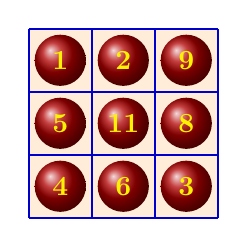
\begin{tikzpicture}[scale=0.8, font=\normalsize]
			\fill[orange!15] (0,0) rectangle (3,3);
			\draw[blue!80!black, thick] (0,0) grid (3,3);
			\tikzset{
				ball/.style={circle, shading=ball, ball color=red!70!black, minimum size=6.5mm, inner sep=0pt, text=yellow, font=\bfseries}
			}
			\node[ball] at (0.5, 2.5) {1};
			\node[ball] at (1.5, 2.5) {2};
			\node[ball] at (2.5, 2.5) {9};
			\node[ball] at (0.5, 1.5) {5};
			\node[ball] at (1.5, 1.5) {11};
			\node[ball] at (2.5, 1.5) {8};
			\node[ball] at (0.5, 0.5) {4};
			\node[ball] at (1.5, 0.5) {6};
			\node[ball] at (2.5, 0.5) {3};
		\end{tikzpicture}
	}
	\par
	\shortans[0]{0,66}
	\loigiai{
		Phép thử là chọn $9$ viên bi từ $11$ viên bi và xếp vào $9$ ô vuông.\\ Số phần tử của không gian mẫu là $n(\Omega) = \mathrm{C}_{11}^9 \cdot 9! = \mathrm{A}_{11}^9$.\\
		Trong $11$ viên bi ban đầu, có $6$ viên bi mang số lẻ (gồm $1; 3; 5; 7; 9; 11$) và $5$ viên bi mang số chẵn (gồm $2; 4; 6; 8; 10$).\\
		Vì phải chọn ra $9$ viên bi nên ta có các trường hợp: $6$ bi lẻ và $3$ bi chẵn; $5$ bi lẻ và $4$ bi chẵn; $4$ bi lẻ và $5$ bi chẵn.\\
		Gọi $A$ là biến cố: \lq\lq Bất kì hàng nào, cột nào cũng có ít nhất một viên bi số lẻ\rq\rq. Ta nhận thấy đếm trực tiếp sẽ rất phức tạp nên ta sử dụng phương pháp phần bù.\\
		Với mỗi bộ $9$ viên bi được chọn, gọi $X$ là tập hợp các cách xếp có ít nhất một hàng không có số lẻ (tức là hàng đó toàn số chẵn); $Y$ là tập hợp các cách xếp có ít nhất một cột không có số lẻ (tức là cột đó toàn số chẵn).\\
		Khi đó, số cách xếp vi phạm yêu cầu bài toán là $n(X \cup Y) = n(X) + n(Y) - n(X \cap Y)$. Vì tính chất đối xứng giữa hàng và cột là như nhau nên chắc chắn có $n(X) = n(Y)$.\\
		Ta xét lần lượt các trường hợp sau:\\
		\textbf{Trường hợp 1:} Chọn $6$ bi lẻ và $3$ bi chẵn. Số cách chọn bi là $\mathrm{C}_5^3 \cdot \mathrm{C}_6^6$.\\
		Khi xếp $6$ bi lẻ vào bảng, ta còn $3$ ô để xếp bi chẵn. Do chỉ có $3$ ô chứa bi chẵn nên không thể tồn tại đồng thời một hàng và một cột đều toàn số chẵn (để có điều này cần ít nhất $5$ ô giao nhau dạng dấu cộng). Suy ra $n(X \cap Y) = 0$.\\
		Để tính $n(X)$, ta chọn ra $1$ hàng (có $\mathrm{C}_3^1$ cách), xếp $3$ số chẵn vào hàng đó (có $3!$ cách), $6$ ô còn lại xếp $6$ số lẻ (có $6!$ cách). Vậy $n(X) = n(Y) = \mathrm{C}_3^1 \cdot 3! \cdot 6! = 12\,960$.\\
		Suy ra $n(X) + n(Y) - n(X \cap Y) = 12\,960 + 12\,960 - 0 = 25\,920$.\\
		Số cách xếp thỏa mãn trong trường hợp này là $\mathrm{C}_5^3 \cdot \mathrm{C}_6^6 \cdot \big[ 9! - 25\,920 \big] = 3\,369\,600$.\\
		\textbf{Trường hợp 2:} Chọn $5$ bi lẻ và $4$ bi chẵn. Số cách chọn bi là $\mathrm{C}_5^4 \cdot \mathrm{C}_6^5$.\\
		Tương tự trường hợp 1, do chỉ có $4$ bi chẵn nên không thể có đồng thời một hàng và một cột toàn số chẵn. Suy ra $n(X \cap Y) = 0$.\\
		Để tính $n(X)$, ta chọn $1$ hàng (có $\mathrm{C}_3^1$ cách), chọn $3$ trong $4$ số chẵn xếp vào hàng đó (có $\mathrm{C}_4^3 \cdot 3!$ cách), $6$ ô còn lại xếp $5$ số lẻ và $1$ số chẵn còn thừa (có $6!$ cách).\\ Vậy $n(X) = n(Y) = \mathrm{C}_3^1 \cdot \mathrm{C}_4^3 \cdot 3! \cdot 6! = 51\,840$.\\
		Suy ra $n(X) + n(Y) - n(X \cap Y) = 51\,840 + 51\,840 - 0 = 103\,680$.\\
		Số cách xếp thỏa mãn trong trường hợp này là $\mathrm{C}_5^4 \cdot \mathrm{C}_6^5 \cdot \left[ 9! - 103\,680 \right] = 7\,776\,000$.\\
		\textbf{Trường hợp 3:} Chọn $4$ bi lẻ và $5$ bi chẵn. Số cách chọn bi là $\mathrm{C}_5^5 \cdot \mathrm{C}_6^4$.\\
		Để tính $n(X)$, ta chọn $1$ hàng (có $\mathrm{C}_3^1$ cách), chọn $3$ trong $5$ số chẵn xếp vào (có $\mathrm{C}_5^3 \cdot 3!$ cách), $6$ ô còn lại xếp $4$ số lẻ và $2$ số chẵn (có $6!$ cách). Vậy $n(X) = n(Y) = \mathrm{C}_3^1 \cdot \mathrm{C}_5^3 \cdot 3! \cdot 6! = 129\,600$.\\
		Tập $X \cap Y$ là các cách xếp có đồng thời $1$ hàng và $1$ cột toàn số chẵn. Ta chọn $1$ hàng và $1$ cột (có $\mathrm{C}_3^1 \cdot \mathrm{C}_3^1$ cách), xếp $5$ số chẵn vào $5$ ô giao nhau này (có $5!$ cách), $4$ ô còn lại xếp $4$ số lẻ (có $4!$ cách). Vậy $n(X \cap Y) = \mathrm{C}_3^1 \cdot \mathrm{C}_3^1 \cdot 5! \cdot 4! = 25\,920$.\\
		Suy ra $n(X) + n(Y) - n(X \cap Y) = 129\,600 + 129\,600 - 25\,920 = 233\,280$.\\
		Số cách xếp thỏa mãn trong trường hợp này là $\mathrm{C}_5^5 \cdot \mathrm{C}_6^4 \cdot \left[ 9! - 233\,280 \right] = 1\,944\,000$.\\
		Tổng số kết quả thuận lợi cho biến cố $A$ là $n(A) = 3\,369\,600 + 7\,776\,000 + 1\,944\,000 = 13\,089\,600$.\\
		Xác suất cần tìm là $\mathrm{P}(A) = \dfrac{n(A)}{n(\Omega)} = \dfrac{13\,089\,600}{\mathrm{A}_{11}^9} \approx 0{,}66$.
	}
\end{ex}
%%%=============================%%%
\Closesolutionfile{ans}

\newpage
\indapan{12}{ans/ansTN-Dung}
\indapan[TF]{2}{ans/ansTN-DungSai}
\indapan[SA]{6}{ans/ansTN-DienKhuyet}
%%%%%%%%%%%%%%
%%nhãn kết thúc đề (để đếm số trang tự động mỗi đề)
\label{B\thedeso}